% =====================================================================
%  Hydroelectric Power Plant Simulation Using OpenGL  -  Project Report
%  Md. Tahmid Islam (2107107), Department of CSE, KUET
%  Build:  pdflatex main.tex   (run it twice so the contents are filled in)
% =====================================================================
\documentclass[11pt,a4paper]{report}

% ---------------------------------------------------------------------
%  Packages
% ---------------------------------------------------------------------
\usepackage[a4paper,top=2.1cm,bottom=2.1cm,left=2.1cm,right=2.1cm,headheight=14pt]{geometry}
\usepackage[T1]{fontenc}
\usepackage{lmodern}
\usepackage{microtype}
\DisableLigatures[-]{family=tt*}   % keep "--" as two dashes in code
\usepackage{graphicx}
\usepackage{amsmath,amssymb}
\usepackage{array,tabularx,longtable,multicol}
\usepackage{float}
\usepackage{caption}
\usepackage{subcaption}
\usepackage{setspace}
\usepackage{enumitem}
\usepackage[dvipsnames]{xcolor}
\usepackage[pagestyles]{titlesec}
\usepackage{tikz}
\usetikzlibrary{arrows.meta,positioning,calc,shapes.geometric,fit,backgrounds}
\usepackage{tcolorbox}
\usepackage{listings}
\usepackage{ragged2e}
\usepackage{hyperref}

% ---------------------------------------------------------------------
%  Colours and general look
% ---------------------------------------------------------------------
\definecolor{accent}{RGB}{18,72,128}
\definecolor{accentlight}{RGB}{232,240,250}
\definecolor{water}{RGB}{40,120,200}
\definecolor{mech}{RGB}{110,118,128}
\definecolor{elec}{RGB}{214,120,30}
\definecolor{codebg}{RGB}{246,247,249}

\hypersetup{
    colorlinks=true, linkcolor=accent, citecolor=accent, urlcolor=accent,
    pdftitle={Hydroelectric Power Plant Simulation Using OpenGL},
    pdfauthor={Md. Tahmid Islam}
}

\graphicspath{{figures/}}
\setstretch{1.04}
\setlength{\parindent}{1.4em}
\setlength{\parskip}{0.2em}
\setlist[itemize]{itemsep=0.15em, topsep=0.3em}
\setlist[enumerate]{itemsep=0.15em, topsep=0.3em}
\captionsetup{font=small, labelfont={bf,color=accent}, margin=0.5cm}
\captionsetup[subfigure]{font=footnotesize, labelfont=bf}
\renewcommand{\arraystretch}{1.2}
% let tables and figures sit on text pages instead of leaving gaps
\renewcommand{\topfraction}{0.9}
\renewcommand{\bottomfraction}{0.7}
\renewcommand{\textfraction}{0.08}
\renewcommand{\floatpagefraction}{0.75}
\makeatletter
\setlength{\@fptop}{0pt}                 % float-only pages start at the top
\setlength{\@fpsep}{14pt}
\setlength{\@fpbot}{0pt plus 1fil}
\makeatother
\setcounter{topnumber}{3}
\setcounter{totalnumber}{4}
\setlength{\textfloatsep}{12pt plus 3pt minus 3pt}
\setlength{\floatsep}{10pt plus 2pt minus 2pt}

% chapter and section headings
\titleformat{\chapter}[display]
  {\normalfont\bfseries\color{accent}}
  {\large\mdseries\scshape \chaptertitlename\ \thechapter}{4pt}{\Huge}
  [\vspace{3pt}{\color{accent}\titlerule[1.2pt]}]
\titlespacing*{\chapter}{0pt}{-24pt}{14pt}
\titlespacing*{\section}{0pt}{1.6ex plus 0.6ex minus 0.3ex}{0.8ex}
\titlespacing*{\subsection}{0pt}{1.3ex plus 0.5ex minus 0.2ex}{0.6ex}
\titleformat{\section}{\normalfont\Large\bfseries\color{accent}}{\thesection}{0.8em}{}
\titleformat{\subsection}{\normalfont\large\bfseries}{\thesubsection}{0.8em}{}
\titleformat{\subsubsection}{\normalfont\normalsize\bfseries}{\thesubsubsection}{0.8em}{}

% running header
\newpagestyle{main}{
  \sethead{\small\itshape Hydroelectric Power Plant Simulation Using OpenGL}{}{\small\thepage}
  \headrule
}
\renewpagestyle{plain}{\setfoot{}{\small\thepage}{}}

% table rules (booktabs-like, built from plain \hline)
\newcommand{\thickhline}{\noalign{\global\setlength{\arrayrulewidth}{0.9pt}}\hline
                         \noalign{\global\setlength{\arrayrulewidth}{0.4pt}}}
\newcommand{\toprule}{\thickhline\noalign{\vskip 2pt}}
\newcommand{\midrule}{\noalign{\vskip 1pt}\hline\noalign{\vskip 2pt}}
\newcommand{\bottomrule}{\noalign{\vskip 1pt}\thickhline}
\newcolumntype{Y}{>{\RaggedRight\arraybackslash}X}
\newcolumntype{L}[1]{>{\RaggedRight\arraybackslash}p{#1}}

% small helpers
\newcommand{\code}[1]{\texttt{\detokenize{#1}}}
\newcommand{\done}{\textcolor{ForestGreen}{\textbf{Completed}}}
\newcommand{\ext}{\textcolor{accent}{\textbf{Extended}}}
\newcommand{\key}[1]{\fbox{\footnotesize\ttfamily #1}}
\newcommand{\vect}[1]{\mathbf{#1}}
\newcommand{\mat}[1]{\mathbf{#1}}
\renewcommand{\bibname}{References}

\newtcolorbox{notebox}[1]{colback=accentlight, colframe=accent, boxrule=0.6pt, arc=2pt,
  left=6pt, right=6pt, top=4pt, bottom=4pt, fonttitle=\bfseries\small, title=#1}

% code listings
\lstset{
  basicstyle=\ttfamily\footnotesize, columns=fullflexible, keepspaces=true,
  backgroundcolor=\color{codebg}, frame=single, rulecolor=\color{black!15},
  keywordstyle=\color{accent}\bfseries, commentstyle=\color{black!55}\itshape,
  numbers=none, xleftmargin=4pt, xrightmargin=4pt, aboveskip=8pt, belowskip=6pt,
  showstringspaces=false, language=C++,
  morekeywords={vec2,vec3,vec4,mat3,mat4,uniform,in,out,float}
}

% ---------------------------------------------------------------------
\begin{document}
% ---------------------------------------------------------------------

% =====================================================================
%  TITLE PAGE
% =====================================================================
\begin{titlepage}
\centering
\vspace*{0.4cm}
{\color{accent}\rule{\textwidth}{1.2pt}}\\[0.5cm]
{\Huge\bfseries Hydroelectric Power Plant\\[0.25cm] Simulation Using OpenGL\par}
\vspace{0.35cm}
{\large\itshape An Interactive 3D Journey from the Reservoir to the Power Grid\par}
\vspace{0.3cm}
{\color{accent}\rule{\textwidth}{1.2pt}}

\vspace{1.1cm}
{\large\textbf{Submitted by}\par}
\vspace{0.2cm}
{\Large Md.\ Tahmid Islam\par}
{\large Roll: 2107107\par}

\vspace{0.9cm}
{\large\textbf{Submitted to}\par}
\vspace{0.2cm}
{\large\textbf{Md Tajmilur Rahman}, Lecturer\par}
{\large\textbf{Md.\ Mubtashim Abrar Nihal}, Lecturer\par}

\vspace{1.0cm}

\includegraphics[width=4.2cm]{kuet-logo.png}

\vfill
{\large Department of Computer Science and Engineering\par}
{\large Khulna University of Engineering \& Technology\par}
{\large Khulna 9203, Bangladesh\par}
\vspace{0.4cm}
{\large 11 October, 2026\par}
\end{titlepage}

% =====================================================================
%  FRONT MATTER
% =====================================================================
\pagenumbering{roman}
\pagestyle{plain}

\chapter*{Abstract}
\addcontentsline{toc}{chapter}{Abstract}

This report describes \emph{HYDRO}, a real-time 3D simulation of a hydroelectric
power plant written in C++ and OpenGL~3.3. The project began as a proposal for a
small ``smart flood sluice gate''. On review, the course teacher asked for the idea
to be grown into a complete hydroelectric power plant, so the gate became one part of
a much larger system. The final program follows a drop of water, and later the
energy it carries, through eleven connected scenes: the reservoir, the trash rack,
the intake gate, the penstock, the main inlet valve, a Francis turbine, the shaft, the
generator, the step-up transformer, and finally the switchyard and power line that
lead to the grid. At every step the viewer takes part: opening the gates, starting
the turbine, exciting the generator and closing the breaker.

Every object is generated in code and every texture is calculated in a shader; no
model files, image files or maths libraries are used. Apart from GLFW (window and
input) and GLAD (loading OpenGL functions), all code, including the matrix library,
the font and the screenshot writer, was written for this project. The program
demonstrates every topic required by the course: Blinn--Phong lighting with
directional and point lights, translation, rotation, scaling, composite and
hierarchical transformations, switchable Gouraud and Phong shading, continuous
physics-based animation, and mouse, keyboard and on-screen interaction. A Whitted-style
ray tracer running on the GPU renders a glass penstock with exact ray--surface
intersections, shadow rays, reflection, refraction and volume ray marching. Shadow
mapping, procedural textures, water rendering, particle systems and a bloom
post-process were added to give the scenes a cinematic look. The plant itself is
driven by one consistent data sheet (53\,m head, 180\,m$^3$/s, 86\,MW, 50\,Hz), and
a cause-and-effect model makes sure that nothing on screen happens before its cause.
The finished program runs at 34--60 frames per second at 1600$\times$900 on a
GTX~1650 laptop GPU.

\begingroup
\hypersetup{linkcolor=black}
\setcounter{tocdepth}{1}
\setstretch{0.97}
% same as report.cls, but with a smaller gap above each chapter entry
\makeatletter
\renewcommand*\l@chapter[2]{%
  \ifnum \c@tocdepth >\m@ne
    \addpenalty{-\@highpenalty}%
    \vskip 0.5em \@plus\p@
    \setlength\@tempdima{1.5em}%
    \begingroup
      \parindent \z@ \rightskip \@pnumwidth
      \parfillskip -\@pnumwidth
      \leavevmode \bfseries
      \advance\leftskip\@tempdima
      \hskip -\leftskip
      #1\nobreak\hfil
      \nobreak\hb@xt@\@pnumwidth{\hss #2\kern-\p@\kern\p@}\par
      \penalty\@highpenalty
    \endgroup
  \fi}
\makeatother
\tableofcontents
\endgroup

% =====================================================================
%  CHAPTER 1  INTRODUCTION
% =====================================================================
\cleardoublepage
\pagenumbering{arabic}
\pagestyle{main}

\chapter{Introduction}

\section{Background}

Bangladesh depends on rivers, and most of us have seen sluice gates and
embankments holding back water during the monsoon. A hydroelectric power plant
takes the same idea much further: instead of only holding water back, it lets the
water fall through a turbine in a controlled way and turns the energy of that fall
into electricity. The path from the lake behind a dam to the socket in a home is
long, and most of it is hidden inside concrete and steel. That makes it a good
subject for computer graphics, where we can cut objects open, slow time down and
show invisible things such as magnetic fields and electric current.

The project tells this story as a live OpenGL program that walks through the plant
in the same order as the water. Instead of only watching, the viewer opens the
gates, starts the turbine, excites the generator and closes the breaker.
Figure~\ref{fig:overview} shows the plant as it appears when the program starts.

\begin{figure}[!htbp]
\centering
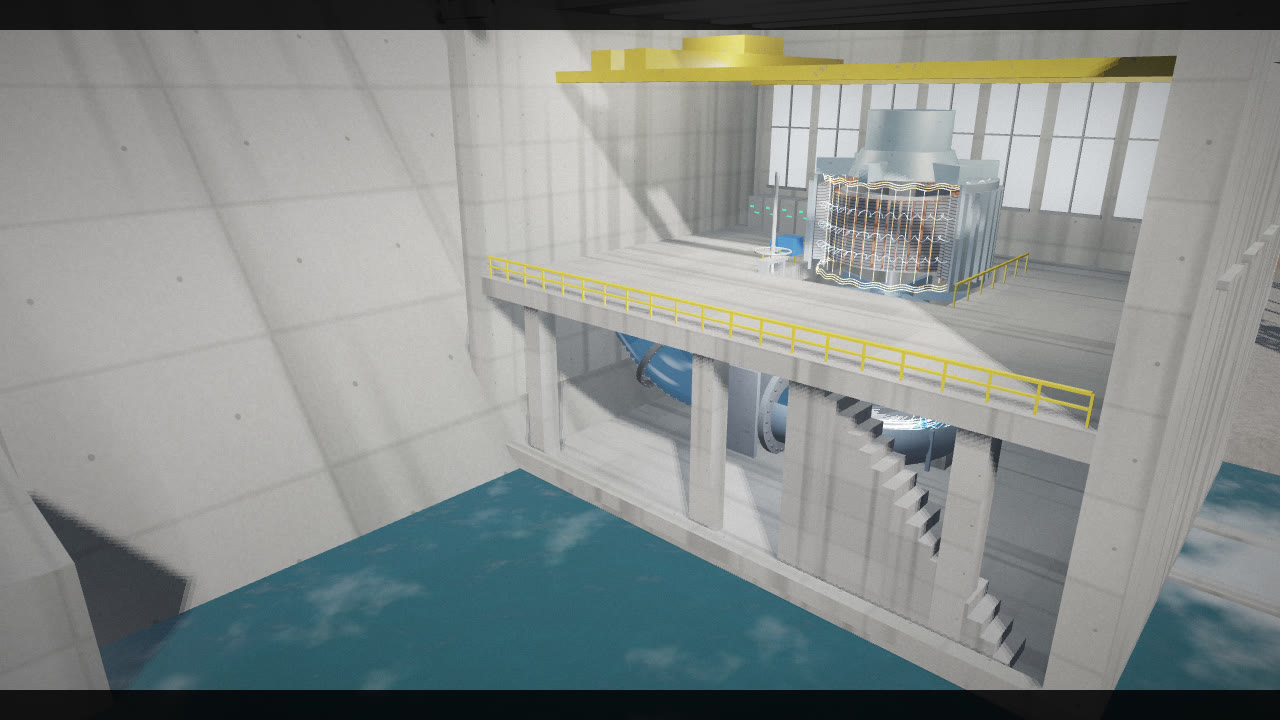
\includegraphics[width=0.78\textwidth]{overview.jpg}
\caption{The running plant: spillway on the left, cut-away powerhouse with the
generator floor and the turbine pit below it.}
\label{fig:overview}
\end{figure}

\section{From a Sluice Gate to a Power Plant}

The original proposal (Appendix~\ref{app:proposal}) was titled \emph{Smart Flood
Sluice Gate}. It described a canal, a movable metal gate, a rotating control wheel,
a changing water level, a floating buoy and warning lights, rendered with Phong
lighting. When the proposal was reviewed, the teacher wrote \emph{``Hydroelectric
Power Plant''} on it and asked for the project to become a hydroelectric plant
simulation.

The two ideas fit together well, because a hydroelectric plant is full of gates,
wheels, shafts and moving water. Every object and feature of the sluice-gate
proposal therefore has a natural place in the power plant: the sluice gate becomes
the intake gate and the spillway gates, the control wheel becomes the hand-wheel of
the main inlet valve, the connecting shaft becomes the turbine--generator shaft, and
the buoy becomes the floating debris stopped by the trash rack. Throughout this
report the \emph{hydroelectric power plant} is treated as the proposed project, and
Chapter~\ref{ch:compare} compares it item by item with what was built.

\section{Objectives}

The main objectives of the project were:
\begin{enumerate}
  \item Build an interactive 3D model of a complete hydroelectric power plant using
        only C++, OpenGL and GLSL, without model files or maths libraries.
  \item Demonstrate the course topics clearly: lighting, transformations, Gouraud and
        Phong shading, motion and animation, user interaction, and ray tracing.
  \item Follow the real order of energy conversion, from potential energy in the
        reservoir to electrical energy in the grid, and keep cause and effect correct.
  \item Give the program a clear, cinematic look: smooth camera moves, cut-away
        views, glowing flow lines and labelled parts.
  \item Keep the code readable, with one file for each object and each scene, so that
        the project is easy to explain and extend.
\end{enumerate}

\section{Tools and Constraints}

The course asked for plain OpenGL in C or C++, without Python and without
third-party libraries. Table~\ref{tab:tools} lists everything the project uses. GLFW
and GLAD are the only external code: GLFW opens the window and reads the keyboard and
mouse, and GLAD looks up the OpenGL functions at run time, which Windows requires for
anything newer than OpenGL~1.1. Neither of them draws anything. Vectors, matrices,
geometry, textures, the font and the image writer are all part of the project.

\begin{table}[!htbp]
\centering
\caption{Tools used in the project.}
\label{tab:tools}
\begin{tabularx}{\textwidth}{@{}L{3.6cm}Y@{}}
\toprule
\textbf{Tool} & \textbf{Purpose} \\
\midrule
C++17 & Main language (about 8\,000 lines in 85 source files). \\
OpenGL 3.3 Core & All rendering~\cite{glspec}. \\
GLSL 3.30 & 21 shader files~\cite{glslspec} (about 1\,300 lines): lighting, water, ray tracer,
            post-processing, user interface. \\
GLFW 3 & Creates the window and the OpenGL context, reports keyboard, mouse and time. \\
GLAD & Generated loader for OpenGL function pointers. \\
MinGW-w64 g++ / CMake & Compiling on Windows (\code{build.bat} or CMake). \\
\midrule
\multicolumn{2}{@{}l}{\textbf{Not used:} GLM, image loaders, model loaders, physics engines,
game engines, Python.} \\
\bottomrule
\end{tabularx}
\end{table}

% =====================================================================
%  CHAPTER 2  PROPOSED VS IMPLEMENTED
% =====================================================================
\chapter{Proposed and Implemented Features}
\label{ch:compare}

This chapter answers a simple question: \emph{was everything that was promised
actually built?} The comparison uses two labels. \done{} means the proposed item is
present and works as described. \ext{} means the item is present and goes clearly
beyond the original description, or that it is a new feature added for the
hydroelectric plant.

\section{Course Requirements}

The course set six compulsory topics. Table~\ref{tab:req} shows where each one is
implemented and how it can be shown during a demonstration.

\begin{table}[!htbp]
\centering
\caption{Compulsory course topics and where they are implemented.}
\label{tab:req}
\small
\begin{tabularx}{\textwidth}{@{}L{2.6cm}L{2.15cm}YL{3.4cm}@{}}
\toprule
\textbf{Topic} & \textbf{Status} & \textbf{Implementation} & \textbf{How to show it} \\
\midrule
Lighting & \ext &
  Blinn--Phong with hemisphere ambient, a directional sun, up to four point lights,
  Fresnel reflections, shadow mapping and under-water light
  (\code{shaders/common.glsl}). &
  Any scene; \key{L} turns shadows on and off. \\
Transformation & \done &
  Own matrix library (\code{MathLib.h}): translation, rotation, scaling, composite and
  hierarchical transforms on gates, valve, 24 guide vanes, runner, rotor, fans and
  debris. &
  Scenes 3, 6 and 7. \\
Gouraud \& Phong shading & \done &
  Two separate shader pairs: \code{gouraud.vert/.frag} (per vertex) and
  \code{lit.vert/.frag} (per pixel). &
  \key{G} cycles Mixed, Phong and Gouraud. \\
Motion / animation & \ext &
  Physics-based water fronts, turbine inertia, buoyant debris, particles, glowing
  flow lines and spline camera paths, all driven by frame time. &
  Every scene; \key{[} \key{]} change the speed. \\
Interaction & \ext &
  On-screen buttons with keyboard shortcuts, mouse orbit, pan and zoom, speed control,
  and buttons that stay locked until their cause has happened. &
  Every scene. \\
Ray tracing & \ext &
  Whitted-style GPU ray tracer with exact intersections, shadow rays, reflection,
  refraction and volume ray marching (\code{shaders/raytrace.frag}). &
  Scene 5; \key{UP}/\key{DOWN} change the head. \\
\bottomrule
\end{tabularx}
\end{table}

\section{Proposed Objects}

Table~\ref{tab:objects} maps each object in the proposal to its form in the power
plant.

\begingroup\small
\begin{longtable}{@{}L{3.5cm}L{2.15cm}L{\dimexpr\textwidth-3.5cm-2.15cm-4\tabcolsep\relax}@{}}
\caption{Objects of the proposal and their implementation in the power plant.}\label{tab:objects}\\
\toprule
\textbf{Proposed object} & \textbf{Status} & \textbf{Implemented as} \\
\midrule
\endfirsthead
\toprule
\textbf{Proposed object} & \textbf{Status} & \textbf{Implemented as} \\
\midrule
\endhead
\bottomrule
\endlastfoot
Canal base and side walls & \ext &
  The water channels of the plant: the reservoir basin, the intake channel, an 11\,m
  wide conduit through the dam, the penstock and the river bed. The valley is a
  260$\times$260 height-field terrain. \\
Movable metal sluice gate & \ext &
  A vertical-lift intake gate with hydraulic cylinders, three spillway gates in the
  dam crest, and the gate of the main inlet valve. \\
Gate frame and vertical support pillars & \ext &
  The intake structure with side piers and a top deck, the gate shaft, the spillway
  piers, and the steel frame of the trash rack. \\
Rotating control wheel and connecting shaft & \ext &
  The hand-wheel of the main inlet valve on its stem, and the main vertical shaft
  that joins the turbine runner to the generator rotor, with a guide bearing and a
  bolted coupling flange. \\
Water surface and water-level indicator & \ext &
  Animated water in the reservoir, river, conduit, penstock and spiral casing, plus
  live read-outs of gate opening, conduit level and casing filling. \\
Floating buoy for showing water movement & \done &
  Floating debris (a branch, logs, crumpled plastic, straw and leaves) that bobs on the
  water and drifts with the current until the trash rack stops it. \\
Warning beacon and light fixture & \done &
  Lamps in the powerhouse (point lights) and red and green status lamps on the circuit
  breakers. \\
Ground area and simple control platform & \ext &
  The valley terrain with boulders, the powerhouse floors with yellow railings, the
  switchyard platform, and the on-screen control panel. \\
Directional and point light sources & \done &
  The sun as a directional light and the powerhouse lamps as point lights with distance
  fall-off. \\
\end{longtable}
\endgroup

\section{Proposed Features}

Table~\ref{tab:features} maps each feature in the proposal to its implementation.

\begingroup\small
\begin{longtable}{@{}L{3.9cm}L{2.15cm}L{\dimexpr\textwidth-3.9cm-2.15cm-4\tabcolsep\relax}@{}}
\caption{Features of the proposal and their implementation.}\label{tab:features}\\
\toprule
\textbf{Proposed feature} & \textbf{Status} & \textbf{Implemented as} \\
\midrule
\endfirsthead
\toprule
\textbf{Proposed feature} & \textbf{Status} & \textbf{Implemented as} \\
\midrule
\endhead
\bottomrule
\endlastfoot
The gate moves vertically to control water flow & \ext &
  The intake gate rises with its piston rods; water jets under it with Torricelli
  speed $\sqrt{2gh}$ and fills the conduit only while it is open. The spillway gates
  and the inlet valve work the same way. \\
The control wheel rotates with its connected shaft & \ext &
  The valve hand-wheel turns only while the valve gate is moving. The runner, shaft
  and generator rotor share one rotation angle, so they turn together. \\
The water level rises and falls dynamically & \ext &
  The conduit level, the penstock water front and the spiral casing filling are
  simulated every frame; closing a gate drains the system again. \\
Floating objects move up and down with the water & \done &
  Each piece of debris is held at its floating depth by a spring--damper buoyancy
  model and bobs with a sine wave. \\
Translation, rotation, scaling, composite and hierarchical transformations & \done &
  All five are used and explained in Section~\ref{sec:transform}. \\
Phong shading with ambient, diffuse and specular reflection & \ext &
  Per-pixel Blinn--Phong, a switchable Gouraud mode, soft shadows, Fresnel reflection
  and tone mapping. \\
User control of the gate, animation speed, lighting and camera & \ext &
  Scene buttons, speed 0.25$\times$ to 2$\times$, shadow, shading and bloom toggles,
  and an orbit, pan and zoom camera on top of the cinematic camera. \\
Reusable primitive meshes keep the scene optimised & \ext &
  A \code{MeshBuilder} creates every shape from a few primitives; one mesh is drawn
  many times with different matrices (24 guide vanes, three spillway gates), and
  hidden parts are culled. \\
\end{longtable}
\endgroup

\section{New Features Added for the Power Plant}

The features in Table~\ref{tab:new} were not in the sluice-gate proposal. They were
added to turn it into the hydroelectric plant the teacher asked for, and they are all
marked \ext.

\begingroup\small
\begin{longtable}{@{}L{4.3cm}L{2.15cm}L{\dimexpr\textwidth-4.3cm-2.15cm-4\tabcolsep\relax}@{}}
\caption{Features added beyond the proposal.}\label{tab:new}\\
\toprule
\textbf{New feature} & \textbf{Status} & \textbf{Summary} \\
\midrule
\endfirsthead
\toprule
\textbf{New feature} & \textbf{Status} & \textbf{Summary} \\
\midrule
\endhead
\bottomrule
\endlastfoot
Complete plant in 11 scenes & \ext & Reservoir to grid in one continuous world with flying camera transitions (Section~\ref{sec:story}). \\
GPU ray tracing & \ext & Whitted ray tracer for the glass penstock (Section~\ref{sec:rt}). \\
Shadow mapping & \ext & 2048$\times$2048 depth map with 3$\times$3 PCF soft edges. \\
Gouraud shading mode & \ext & A second lighting path evaluated per vertex, switchable at run time. \\
Procedural textures & \ext & 15 material patterns from noise: concrete, steel, copper, rock, bark and more. \\
Water rendering & \ext & Sine-sum waves, Fresnel reflection, Snell's window, caustics and under-water fog. \\
Particle systems & \ext & Six systems for spray, mist, foam, splashes, gate spray and under-water dust. \\
Flow-line visualisation & \ext & Glowing pulses for water streamlines, magnetic field, current and the power line. \\
Turbine, generator, transformer, switchyard & \ext & Detailed machines with working cause and effect. \\
Physically based plant data & \ext & $P=\rho gQH\eta$, $f=pn/120$ and other formulas drive every number on screen. \\
Cinematic cameras & \ext & Catmull--Rom camera paths with continuity between scenes. \\
Post-processing & \ext & Bloom, vignette and film grain; cross-dissolves between render styles. \\
Information display & \ext & Telemetry panel, 3D pointer labels, an oscilloscope and an energy summary, drawn with a hand-made pixel font. \\
Cut-away and X-ray views & \ext & Parts of the dam, intake, pipe, valve, casing and generator open up for viewing. \\
Testing tools & \ext & Scripted screenshots, an automatic play-through test and a benchmark mode. \\
\end{longtable}
\endgroup

\begin{notebox}{In short}
All six compulsory topics are present, every object and feature of the proposal has
been implemented in the hydroelectric plant, and fifteen new features were added on
top.
\end{notebox}

% =====================================================================
%  CHAPTER 3  SYSTEM DESIGN
% =====================================================================
\chapter{System Design}
\label{ch:design}

\section{Architecture}

The program is organised in layers (Figure~\ref{fig:arch}). \code{main.cpp} reads
the command line and starts the \code{App}. The \code{App} owns the window, the
input, the scene list, the transitions and the user interface. Each of the eleven
\emph{scenes} is a small class that only decides what the camera does, which buttons
are offered and which labels are shown. All the actual content lives in a single
\code{World} object, which builds the whole plant once and runs the simulation. The
world is made of \emph{objects}, one file per object, and the objects draw themselves
through the \code{Renderer}, which talks to the GLSL shaders.

\begin{figure}[!htbp]
\centering
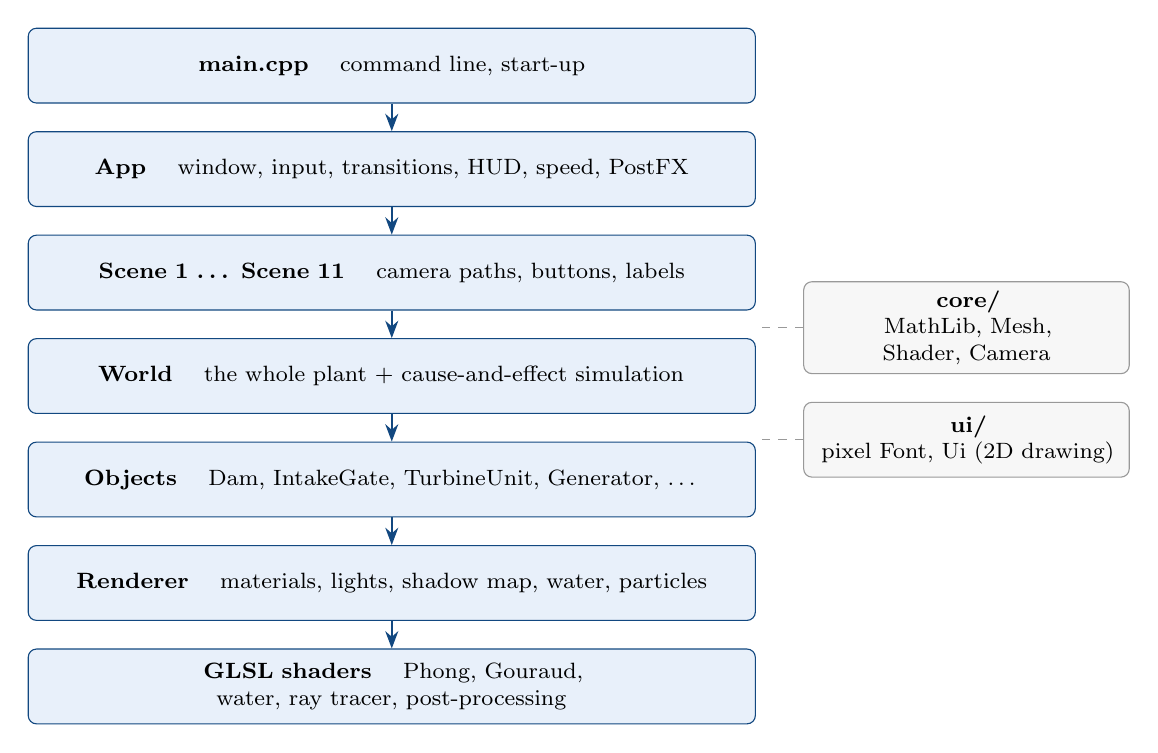
\begin{tikzpicture}[
  layer/.style={draw=accent, fill=accentlight, rounded corners=3pt, text width=9.0cm,
                minimum height=0.95cm, align=center, font=\footnotesize},
  side/.style={draw=black!40, fill=black!3, rounded corners=3pt, text width=3.9cm,
               minimum height=0.95cm, align=center, font=\footnotesize},
  arr/.style={-{Stealth[length=2.2mm]}, thick, accent}]
\node[layer] (main) {\textbf{main.cpp} \quad command line, start-up};
\node[layer, below=0.35cm of main] (app) {\textbf{App} \quad window, input, transitions, HUD, speed, PostFX};
\node[layer, below=0.35cm of app] (scenes) {\textbf{Scene 1 \dots\ Scene 11} \quad camera paths, buttons, labels};
\node[layer, below=0.35cm of scenes] (world) {\textbf{World} \quad the whole plant + cause-and-effect simulation};
\node[layer, below=0.35cm of world] (objects) {\textbf{Objects} \quad Dam, IntakeGate, TurbineUnit, Generator, \dots};
\node[layer, below=0.35cm of objects] (renderer) {\textbf{Renderer} \quad materials, lights, shadow map, water, particles};
\node[layer, below=0.35cm of renderer] (shaders) {\textbf{GLSL shaders} \quad Phong, Gouraud, water, ray tracer, post-processing};
\foreach \a/\b in {main/app, app/scenes, scenes/world, world/objects, objects/renderer, renderer/shaders}
  \draw[arr] (\a) -- (\b);
\node[side, right=0.6cm of scenes, yshift=-0.7cm] (core) {\textbf{core/}\\ MathLib, Mesh, Shader, Camera};
\node[side, below=0.35cm of core] (ui) {\textbf{ui/}\\ pixel Font, Ui (2D drawing)};
\draw[black!40, dashed] (core.west) -- ++(-0.6,0);
\draw[black!40, dashed] (ui.west) -- ++(-0.6,0);
\end{tikzpicture}
\caption{Layered architecture of the program.}
\label{fig:arch}
\end{figure}

Because every scene looks at the same \code{World}, nothing is duplicated. The water
the viewer releases at the intake gate is the same water that later fills the spiral
casing, and the turbine that spins in the preview is the same turbine that is
examined in scene~7. Table~\ref{tab:modules} lists the main modules.

\begin{table}[!htbp]
\centering
\caption{Main modules and their responsibilities.}
\label{tab:modules}
\begin{tabularx}{\textwidth}{@{}L{5.25cm}Y@{}}
\toprule
\textbf{Module} & \textbf{Responsibility} \\
\midrule
\code{core/MathLib.h} & Vectors, 4$\times$4 matrices, all transformation and camera matrices. \\
\code{core/Mesh.cpp} & GPU buffers (VAO, VBO, EBO) and the \code{MeshBuilder} that generates shapes. \\
\code{core/Shader.cpp} & Compiles shaders and expands a simple \texttt{\#include} so shaders can share code. \\
\code{core/Camera.cpp} & Look-at camera, user orbit and Catmull--Rom camera paths. \\
\code{render/Renderer.cpp} & Lights, materials, shadow pass, choice of Phong or Gouraud shader. \\
\code{render/ParticleSystem.cpp} & Particle update and camera-facing billboards. \\
\code{render/PostFX.cpp} & Bloom, vignette and film grain. \\
\code{render/FrameCapture.cpp} & Keeps the last frame for cross-dissolves. \\
\code{objects/World.cpp} & Builds the plant, runs the simulation, draws in the right order, culls. \\
\code{objects/PlantData.h} & The plant's data sheet and formulas. \\
\code{objects/*.cpp} (18 files) & One file per object (Chapter~\ref{ch:objects}). \\
\code{scenes/*.cpp} (11 files) & One file per scene (Chapter~\ref{ch:walk}). \\
\code{ui/Font.cpp}, \code{ui/Ui.cpp} & Hand-made 5$\times$7 pixel font and 2D drawing of the HUD. \\
\bottomrule
\end{tabularx}
\end{table}

\section{The Story: Eleven Connected Scenes}
\label{sec:story}

The program follows the real path of energy through the plant. Water carries
potential energy from the reservoir, turns it into kinetic energy in the penstock and
mechanical energy in the turbine, and the generator turns that into electrical
energy, which the transformer and the switchyard send to the grid
(Figure~\ref{fig:story}).

\begin{figure}[!htbp]
\centering
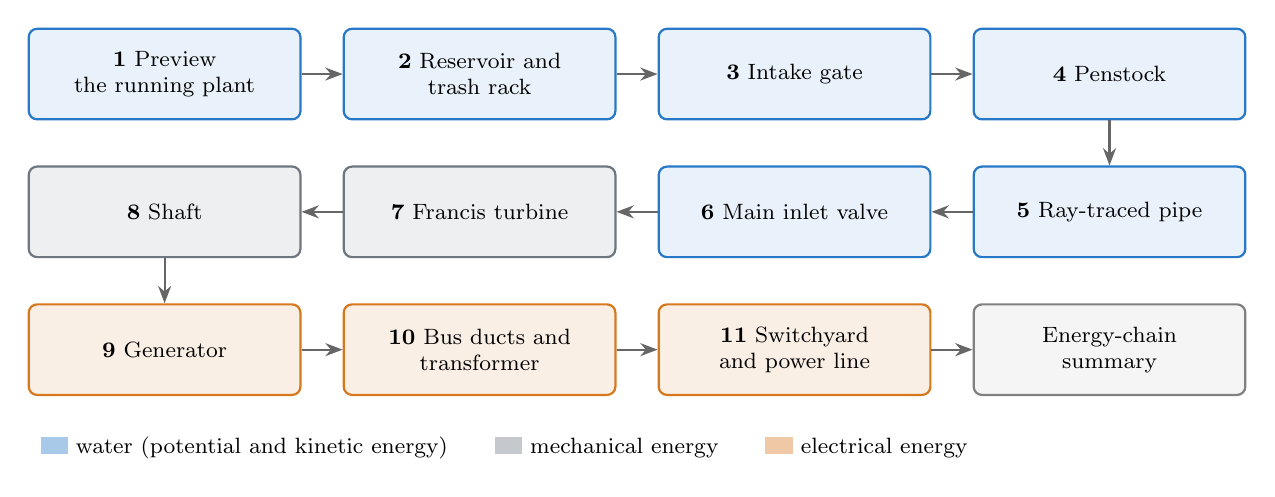
\begin{tikzpicture}[
  st/.style={draw, rounded corners=3pt, minimum width=3.45cm, minimum height=1.15cm,
             align=center, font=\footnotesize, line width=0.8pt},
  w/.style={st, draw=water, fill=water!10},
  m/.style={st, draw=mech, fill=mech!12},
  e/.style={st, draw=elec, fill=elec!12},
  arr/.style={-{Stealth[length=2.2mm]}, thick, black!60}]
\node[w] (s1) at (0,0) {\textbf{1} Preview\\ the running plant};
\node[w] (s2) at (4,0) {\textbf{2} Reservoir and\\ trash rack};
\node[w] (s3) at (8,0) {\textbf{3} Intake gate};
\node[w] (s4) at (12,0) {\textbf{4} Penstock};
\node[w] (s5) at (12,-1.75) {\textbf{5} Ray-traced pipe};
\node[w] (s6) at (8,-1.75) {\textbf{6} Main inlet valve};
\node[m] (s7) at (4,-1.75) {\textbf{7} Francis turbine};
\node[m] (s8) at (0,-1.75) {\textbf{8} Shaft};
\node[e] (s9) at (0,-3.5) {\textbf{9} Generator};
\node[e] (s10) at (4,-3.5) {\textbf{10} Bus ducts and\\ transformer};
\node[e] (s11) at (8,-3.5) {\textbf{11} Switchyard\\ and power line};
\node[st, draw=black!50, fill=black!4] (sum) at (12,-3.5) {Energy-chain\\ summary};
\draw[arr] (s1) -- (s2); \draw[arr] (s2) -- (s3); \draw[arr] (s3) -- (s4);
\draw[arr] (s4) -- (s5); \draw[arr] (s5) -- (s6); \draw[arr] (s6) -- (s7);
\draw[arr] (s7) -- (s8); \draw[arr] (s8) -- (s9); \draw[arr] (s9) -- (s10);
\draw[arr] (s10) -- (s11); \draw[arr] (s11) -- (sum);
\node[font=\footnotesize, anchor=west] at (-1.7,-4.75)
  {\textcolor{water!40}{\rule{0.35cm}{0.22cm}}\ water (potential and kinetic energy)\qquad
   \textcolor{mech!40}{\rule{0.35cm}{0.22cm}}\ mechanical energy\qquad
   \textcolor{elec!40}{\rule{0.35cm}{0.22cm}}\ electrical energy};
\end{tikzpicture}
\caption{The eleven scenes follow the energy through the plant.}
\label{fig:story}
\end{figure}

The scenes are not separate levels. When the viewer presses a \emph{follow} button,
the current camera position is handed to the next scene (\code{App::continueTo}),
and the next camera path starts exactly there, so the camera keeps flying. Only
where the rendering style changes completely (from under water to a cut-away
diagram, or from rasterisation to ray tracing) does the program cross-dissolve
instead. Table~\ref{tab:scenes} lists the scenes and their controls.

\begin{table}[!htbp]
\centering
\caption{The eleven scenes and their controls.}
\label{tab:scenes}
\small
\begin{tabularx}{\textwidth}{@{}L{0.4cm}L{2.9cm}YL{4.0cm}@{}}
\toprule
\textbf{\#} & \textbf{Scene} & \textbf{What happens} & \textbf{Controls} \\
\midrule
1 & Preview & The finished plant at work: spillway, cut-away powerhouse, spinning machines. & Stop/start water \key{SPACE}, show water movement \key{ENTER} \\
2 & Reservoir and trash rack & Camera flies over the dam and dives to the intake; trash piles up at the rack. & Add more trash \key{T}, follow \\
3 & Intake gate & The dam block lifts away; the gate opens and the conduit fills. & Open gate \key{O}; follow unlocks when fully open \\
4 & Penstock & Water rushes down the pipe and stops at the closed valve. & X-ray \key{X}, replay flow, follow \\
5 & Ray-traced pipe & Ray-traced glass penstock with glowing water. & Head \key{UP} \key{DOWN}, follow \\
6 & Main inlet valve & The valve opens and the spiral casing fills. & Open valve \key{O}; follow unlocks when full \\
7 & Francis turbine & Guide vanes open and the runner speeds up to 150\,rpm. & Guide vanes \key{O}, section \key{X}; follow unlocks at 140\,rpm \\
8 & Shaft & Hologram-style rise along the turning shaft. & Automatic \\
9 & Generator & Exciting the rotor creates a field and three-phase current. & Excite rotor \key{O}; follow unlocks at 10.5\,kV \\
10 & Transformer & Bus ducts carry 11\,kV; the transformer raises it to 220\,kV. & X-ray \key{X}, follow \\
11 & Switchyard and grid & Closing the breaker sends power along the line; summary appears. & Breaker \key{O}, replay journey \\
\bottomrule
\end{tabularx}
\end{table}

\section{The Frame Pipeline}

Every frame goes through the same steps (Figure~\ref{fig:frame}). The scene first
advances its story by $\Delta t \times \text{speed}$, where $\Delta t$ is the measured
frame time, limited to 0.05\,s so that a paused window cannot produce one huge
physics step. The world is then drawn twice: once from the sun into the shadow map,
and once from the camera into an off-screen colour texture. That texture goes
through the post-processing passes, is copied for a possible dissolve, and finally
the HUD is drawn on top.

\begin{figure}[!htbp]
\centering
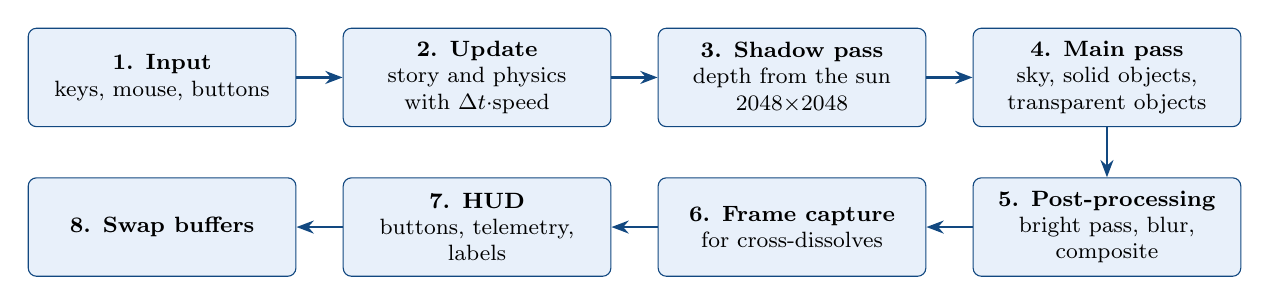
\begin{tikzpicture}[
  bx/.style={draw=accent, fill=accentlight, rounded corners=3pt, minimum width=3.4cm,
             minimum height=1.25cm, align=center, font=\footnotesize},
  arr/.style={-{Stealth[length=2.2mm]}, thick, accent}]
\node[bx] (a) at (0,0) {\textbf{1. Input}\\ keys, mouse, buttons};
\node[bx] (b) at (4,0) {\textbf{2. Update}\\ story and physics\\ with $\Delta t\cdot$speed};
\node[bx] (c) at (8,0) {\textbf{3. Shadow pass}\\ depth from the sun\\ 2048$\times$2048};
\node[bx] (d) at (12,0) {\textbf{4. Main pass}\\ sky, solid objects,\\ transparent objects};
\node[bx] (e) at (12,-1.9) {\textbf{5. Post-processing}\\ bright pass, blur,\\ composite};
\node[bx] (f) at (8,-1.9) {\textbf{6. Frame capture}\\ for cross-dissolves};
\node[bx] (g) at (4,-1.9) {\textbf{7. HUD}\\ buttons, telemetry,\\ labels};
\node[bx] (h) at (0,-1.9) {\textbf{8. Swap buffers}};
\draw[arr] (a)--(b); \draw[arr] (b)--(c); \draw[arr] (c)--(d); \draw[arr] (d)--(e);
\draw[arr] (e)--(f); \draw[arr] (f)--(g); \draw[arr] (g)--(h);
\end{tikzpicture}
\caption{Steps of one frame.}
\label{fig:frame}
\end{figure}

Inside the main pass the order matters. The sky is drawn first, then all opaque
objects with depth writing on, then transparent objects (water, glass, glowing
lines, particles) with blending and depth writing off, so that they blend over what
is already behind them.

\section{The Plant Model}

\subsection{One data sheet}

Early versions showed numbers that did not agree with each other: a flow that did
not match the power, or an rpm that did not match the frequency. The final program
takes every number from one data sheet, \code{objects/PlantData.h}
(Table~\ref{tab:plant}), so all read-outs are consistent.

\begin{table}[!htbp]
\centering
\caption{The plant data sheet.}
\label{tab:plant}
\begin{tabular}{@{}lll@{}}
\toprule
\textbf{Quantity} & \textbf{Value} & \textbf{Comment} \\
\midrule
Reservoir level, tail-water level & 56\,m, 3\,m & world coordinates \\
Gross head $H$ & 53\,m & $56-3$ \\
Flow through one unit $Q$ & 180\,m$^3$/s & at full guide-vane opening \\
Overall efficiency $\eta$ & 0.92 & \\
Rated power $P$ & 86\,MW & $\rho g Q H \eta$ \\
Turbine and generator speed $n$ & 150\,rpm & \\
Generator poles $p$ & 40 & \\
Frequency $f$ & 50\,Hz & $p\,n/120$ \\
Generator voltage, grid voltage & 11\,kV, 220\,kV & transformer ratio 1\,:\,20 \\
\bottomrule
\end{tabular}
\end{table}

\subsection{Plant equations}

The hydraulic power available from water falling through a head $H$ is
\begin{equation}
  P = \rho\, g\, Q\, H\, \eta = 1000 \times 9.81 \times 180 \times 53 \times 0.92
    \approx 86.1\ \text{MW},
  \label{eq:power}
\end{equation}
where $\rho$ is the density of water and $g$ the gravitational acceleration. The
torque on the shaft follows from $P = T\omega$:
\begin{equation}
  T = \frac{P}{\omega} = \frac{P}{2\pi n/60}
    = \frac{86\times10^{6}}{15.71} \approx 5.5\ \text{MN\,m}.
\end{equation}
A synchronous generator with $p$ poles turning at $n$ rpm produces~\cite{chapman}
\begin{equation}
  f = \frac{p\, n}{120} = \frac{40 \times 150}{120} = 50\ \text{Hz}.
  \label{eq:freq}
\end{equation}
For three-phase power the line current is $I = P/(\sqrt{3}\,V)$, which gives
4.5\,kA at 11\,kV and only 0.23\,kA at 220\,kV. This is why the transformer steps the
voltage up: the same power travels with twenty times less current, and the resistive
loss $I^2R$ falls by a factor of four hundred. The ideal speed of water falling through
the full head is $v=\sqrt{2gH}\approx 32$\,m/s.

The 3D rotor turns more slowly than 150\,rpm so that the eye can follow it. The
program keeps a visual angular speed $\omega_v$ and converts it back for the
read-outs with $n = 150\,\omega_v/\Omega_v$, where $\Omega_v = 2.4$\,rad/s is the
visual speed at full load.

\subsection{Cause and effect}

A rule set for the whole project was that \emph{nothing happens before its cause}.
\code{World::update} enforces the chain in Table~\ref{tab:cause}. Because of it, the
viewer cannot reach a state that would be physically wrong, such as voltage from a
stopped rotor or power flowing through an open breaker.

\begin{table}[!htbp]
\centering
\caption{Cause-and-effect rules in the simulation.}
\label{tab:cause}
\begin{tabularx}{\textwidth}{@{}L{4.6cm}Y@{}}
\toprule
\textbf{Effect} & \textbf{Requires} \\
\midrule
Conduit fills & intake gate open \\
Penstock fills & conduit full \\
Spiral casing fills & main inlet valve more than 30\,\% open and penstock full \\
Water flows through the runner & casing full and valve open; the flow equals the guide-vane opening \\
Runner speeds up & water flowing; speed follows the flow with inertia \\
Voltage appears & $V = 11\,\text{kV}\times(\text{field current})\times\min(1, n/150)$ \\
Power line becomes live & breaker closed and $V > 9$\,kV \\
Power is delivered & breaker closed; $P=\rho g (Q\,q) H\eta$ with $q$ the opening \\
\bottomrule
\end{tabularx}
\end{table}

When the viewer jumps straight to a later scene with the number keys,
\code{World::completeUpTo} performs every earlier step instantly, so the scene still
starts in a correct state.

% =====================================================================
%  CHAPTER 4  GRAPHICS THEORY AND IMPLEMENTATION
% =====================================================================
\chapter{Graphics Theory and Implementation}
\label{ch:theory}

This chapter explains each graphics feature in three parts: the idea, the equations
behind it, and how the project implements it. General background comes from
Foley et al.~\cite{foley} and \emph{Real-Time Rendering}~\cite{rtr}.

\section{Geometry and Procedural Modelling}
\label{sec:geometry}

No model files are loaded. Every object is built at start-up by a \code{MeshBuilder}
(\code{core/Mesh.cpp}) that knows a small set of primitives:

\begin{itemize}
  \item \textbf{quads and boxes} for walls, floors, beams and tanks;
  \item \textbf{cylinders and cones} with optional caps and partial angles (for
        cut-aways), plus a helper that stands a cylinder between two points;
  \item \textbf{spheres, tori, disks and annuli} for bearings, bolts, rings and flanges;
  \item \textbf{grids} for terrain and water surfaces;
  \item \textbf{sweeps}: a circle swept along a path with rounded corners, used for the
        penstock, the spiral casing, bus ducts and flow lines;
  \item \textbf{extruded outlines}: a 2D profile pushed along an axis, used for the
        cross-section of the gravity dam.
\end{itemize}

Each vertex stores a position, a normal and a texture coordinate (32 bytes). The
builder holds a current transformation matrix $\mat{M}$: every shape added is
multiplied by $\mat{M}$ and its normals by the normal matrix of $\mat{M}$. This means
a complex part can be assembled by placing simple shapes, exactly as a modeller would.
For example, the 72 stator slots of the generator are one slot shape added 72 times
with $\mat{M} = \mat{T}(\text{centre})\,\mat{R}_y(2\pi k/72)$. Texture coordinates are
measured in metres, so procedural textures have the same scale on every object.

The finished vertices are uploaded once into a vertex buffer and an index buffer.
Meshes that change every frame (the conduit water surface) are created with
\code{GL_DYNAMIC_DRAW} and updated with \code{glBufferSubData}.

\section{Transformations}
\label{sec:transform}

\subsection{Homogeneous matrices}

Points are written in homogeneous coordinates $\vect{p} = (x, y, z, 1)^T$ so that
translation, rotation and scaling can all be expressed as $4\times4$ matrices and
combined by multiplication~\cite{foley}. The matrix library \code{core/MathLib.h}
stores them in column-major order, which is the layout OpenGL expects. The basic
matrices are
\begin{equation}
\mat{T}(t)=\begin{bmatrix}1&0&0&t_x\\0&1&0&t_y\\0&0&1&t_z\\0&0&0&1\end{bmatrix},\qquad
\mat{S}(s)=\begin{bmatrix}s_x&0&0&0\\0&s_y&0&0\\0&0&s_z&0\\0&0&0&1\end{bmatrix},
\end{equation}
\begin{equation}
\mat{R}_x(\theta)=\begin{bmatrix}1&0&0&0\\0&\cos\theta&-\sin\theta&0\\0&\sin\theta&\cos\theta&0\\0&0&0&1\end{bmatrix},\qquad
\mat{R}_y(\theta)=\begin{bmatrix}\cos\theta&0&\sin\theta&0\\0&1&0&0\\-\sin\theta&0&\cos\theta&0\\0&0&0&1\end{bmatrix},
\end{equation}
\begin{equation}
\mat{R}_z(\theta)=\begin{bmatrix}\cos\theta&-\sin\theta&0&0\\\sin\theta&\cos\theta&0&0\\0&0&1&0\\0&0&0&1\end{bmatrix}.
\end{equation}
Rotation about an arbitrary unit axis $\vect{a}$ uses Rodrigues' formula,
\begin{equation}
\mat{R}_{\vect{a}}(\theta) = \cos\theta\,\mat{I} + (1-\cos\theta)\,\vect{a}\vect{a}^T + \sin\theta\,[\vect{a}]_\times ,
\end{equation}
where $[\vect{a}]_\times$ is the cross-product matrix of $\vect{a}$. A helper
\code{alignY} builds an orthonormal basis whose $y$ axis points along a given
direction; it is used to stand cylinders between two points, for example bolts,
pipes and insulators.

\subsection{Composite and hierarchical transformations}

A model matrix is usually a product of several basic matrices. With column vectors
the right-most matrix acts first, so
\begin{equation}
\mat{M} = \mat{T}\,\mat{R}\,\mat{S}
\end{equation}
first scales the object, then rotates it, and finally moves it into place. In a
\emph{hierarchy}, a child part is defined relative to its parent, and its world matrix
is the parent's matrix times its own local matrix:
$\mat{M}_{\text{child}} = \mat{M}_{\text{parent}}\,\mat{M}_{\text{local}}$. Moving
the parent automatically moves every child. Table~\ref{tab:transforms} lists the
transformations used in the plant.

\begin{table}[!htbp]
\centering
\caption{Transformations used on the moving parts.}
\label{tab:transforms}
\begin{tabularx}{\textwidth}{@{}L{3.3cm}L{5.1cm}Y@{}}
\toprule
\textbf{Part} & \textbf{Matrix} & \textbf{Type} \\
\midrule
Spillway gates (3) & $\mat{T}(\text{bay}_i + h\,\hat{\vect{y}})$ & one mesh, three translations \\
Dam cut-away block & $\mat{T}(0,\ 160\,e(\text{lift}),\ 0)$ & translation with easing \\
Intake gate and rods & $\mat{M}_{\text{base}}\,\mat{T}(0,h,0)$ & hierarchical: rods follow the gate \\
Valve gate and stem & $\mat{T}(0,\ 4.4\,u,\ 0)$ & translation \\
Valve hand-wheel & $\mat{T}(\text{top})\,\mat{R}_y(\phi)$ & composite \\
Guide vanes (24) & $\mat{T}(\vect{p}_k)\,\mat{R}_y(-(\theta_k + 90^\circ + \beta))$ & composite; each vane turns about its own pivot \\
Runner, shaft, rotor & $\mat{T}(\vect{c})\,\mat{R}_y(\alpha)$ & composite; one shared angle \\
Transformer fans (4) & $\mat{T}(\vect{f}_i)\,\mat{R}_z(\phi)$ & composite \\
Floating debris & $\mat{P}\,\mat{T}(\vect{x})\,\mat{R}_y\mat{R}_z\mat{R}_x\,\mat{S}(s)$ & hierarchical, with scaling \\
\bottomrule
\end{tabularx}
\end{table}

The intake gate is the clearest example of a hierarchy. The gate leaf and the piston
rods that lift it are drawn with the same matrix, so the rods slide into their fixed
cylinders as the gate rises:

\begin{lstlisting}
// IntakeGate::draw - the rods are attached to the leaf, so they use its matrix
Mat4 up = base * translate(Vec3(0, lift, 0));
r.drawMesh(leaf, up, paint);
r.drawMesh(rods, up, steel);        // rods move WITH the gate
r.drawMesh(cylinders, base, paint); // cylinders stay where they are
\end{lstlisting}

The debris uses a two-level hierarchy. Each piece is simulated in a local ``flow
frame'' in which the current always runs along $+x$. The parent matrix $\mat{P}$ then
places that frame at the trash rack in the world, so the physics code stays simple.

The 24 guide vanes show a composite transformation clearly. All vanes share one mesh.
Vane $k$ is moved to its pivot $\vect{p}_k$ on a circle of radius 1.98\,m and turned
about the vertical axis by its position angle $\theta_k = 2\pi k/24$ plus the opening
angle $\beta = 8^\circ + 38^\circ\times\text{opening}$. Changing one number, the
opening, turns all 24 vanes together, like the operating ring of a real turbine.

\subsection{Normal transformation}

Normals cannot simply be multiplied by the model matrix when the matrix contains
non-uniform scaling, because they would no longer be perpendicular to the surface.
The correct normal matrix is the inverse transpose of the upper $3\times3$ part,
\begin{equation}
\mat{N} = \left(\mat{M}_{3\times3}^{-1}\right)^{T},
\end{equation}
which \code{normalMatrix} computes with the adjugate formula.

\subsection{Viewing and projection}

A point goes from object space to clip space through
\begin{equation}
\vect{p}_{\text{clip}} = \mat{P}\,\mat{V}\,\mat{M}\,\vect{p}_{\text{local}} .
\end{equation}
The view matrix $\mat{V}$ is built by \code{lookAt}. From the eye $\vect{e}$, the
target $\vect{t}$ and the world up vector, it forms the forward vector
$\vect{f}=\text{normalize}(\vect{t}-\vect{e})$, the side vector
$\vect{s}=\text{normalize}(\vect{f}\times\vect{up})$ and the true up vector
$\vect{u}=\vect{s}\times\vect{f}$, and uses them as the rows of a rotation followed by a
translation by $-\vect{e}$. The perspective matrix, for a vertical field of view
$\varphi$, aspect ratio $a$ and near and far planes $n$ and $f$, is
\begin{equation}
\mat{P}=\begin{bmatrix}
\frac{c}{a}&0&0&0\\[2pt] 0&c&0&0\\[2pt] 0&0&\frac{f+n}{n-f}&\frac{2fn}{n-f}\\[2pt] 0&0&-1&0
\end{bmatrix},\qquad c = \frac{1}{\tan(\varphi/2)} .
\end{equation}
The shadow pass uses an orthographic matrix instead, because sunlight is parallel.

\section{Camera System}

The camera has two layers. The \emph{director's camera} is scripted by each scene as a
list of key positions $(t_i, \vect{e}_i, \vect{t}_i)$, and the eye and target are
interpolated with a Catmull--Rom spline~\cite{catmull}. For the segment between keys
$\vect{P}_1$ and $\vect{P}_2$ with neighbours $\vect{P}_0$ and $\vect{P}_3$,
\begin{equation}
\vect{C}(u) = \tfrac12\Big[2\vect{P}_1 + (\vect{P}_2-\vect{P}_0)\,u
 + (2\vect{P}_0-5\vect{P}_1+4\vect{P}_2-\vect{P}_3)\,u^2
 + (-\vect{P}_0+3\vect{P}_1-3\vect{P}_2+\vect{P}_3)\,u^3\Big],\quad u\in[0,1].
\end{equation}
The curve passes through every key and has a continuous tangent, so the camera glides
through the keys like a real crane shot instead of stopping at each one. On the first
and last segments $u$ is replaced by $u' = \tfrac12(3u^2-2u^3)+\tfrac12u$, which eases
the motion in and out.

The second layer is the \emph{user orbit}. Dragging the mouse changes a yaw $\psi$ and a
pitch $\vartheta$ around the target, the wheel changes a zoom factor $z$, and the
keyboard adds a pan vector. The final eye position is
\begin{equation}
\vect{e}' = \vect{t} + \vect{pan} + z\,d\,(\sin\psi\cos\vartheta,\ \sin\vartheta,\ \cos\psi\cos\vartheta),
\end{equation}
with the pitch limited to $[-80^\circ, 85^\circ]$. Pressing \key{C} resets the orbit
and returns to the director's camera.

\section{Lighting}
\label{sec:lighting}

\subsection{The Phong reflection model}

The Phong model~\cite{phong} splits the light reflected from a surface into three
parts. \emph{Ambient} light is a constant that stands for light bouncing around the
scene. \emph{Diffuse} light depends on how directly the surface faces the light,
following Lambert's cosine law. \emph{Specular} light is the shiny highlight that
appears where the reflection of the light points towards the eye. With the unit
normal $\vect{N}$, the direction to the light $\vect{L}$, the direction to the viewer
$\vect{V}$ and the reflected light direction $\vect{R} = 2(\vect{N}\cdot\vect{L})\vect{N}-\vect{L}$,
\begin{align}
I_a &= k_a\, I_{\text{amb}}, \label{eq:amb}\\
I_d &= k_d\, I_L\, \max(\vect{N}\cdot\vect{L},\,0), \label{eq:diff}\\
I_s &= k_s\, I_L\, \max(\vect{R}\cdot\vect{V},\,0)^{n}, \label{eq:spec}\\
I &= I_a + \sum_{\text{lights}} \left(I_d + I_s\right), \label{eq:phong}
\end{align}
where $k_a$, $k_d$, $k_s$ are the material's ambient, diffuse and specular
coefficients, $I_L$ is the light's colour and $n$ is the shininess: a larger $n$ gives
a smaller, sharper highlight.

\subsection{Blinn--Phong as used in the project}

The project uses Blinn's variant~\cite{blinn}, which replaces $\vect{R}\cdot\vect{V}$
with $\vect{N}\cdot\vect{H}$, where $\vect{H}$ is the halfway vector between the light
and the eye:
\begin{equation}
\vect{H} = \frac{\vect{L}+\vect{V}}{\lVert\vect{L}+\vect{V}\rVert},\qquad
I_s = k_s\,\frac{n+8}{32}\,I_L\,\max(\vect{N}\cdot\vect{H},0)^{n}.
\end{equation}
The highlight looks more natural at grazing angles and is cheaper to compute. The
factor $(n+8)/32$ is a normalisation, scaled so that $n=24$ gives a factor of one: it
keeps a sharp highlight bright and a broad one dim, so changing the shininess does
not change the total amount of reflected light much. The complete lighting function,
\code{shade()} in \code{shaders/common.glsl}, adds four more terms to
Equation~\eqref{eq:phong}:

\begin{itemize}
  \item \textbf{Hemisphere ambient.} Instead of a flat constant, the ambient colour
        blends from the ground colour to the sky colour according to which way the
        surface faces:
        $I_a = k_d\, I_{\text{amb}}\cdot\text{mix}\!\left(C_{\text{ground}},\,C_{\text{sky}},\,\tfrac{N_y+1}{2}\right)$.
        Surfaces facing up look bluer and surfaces facing down look warmer.
  \item \textbf{Shadows.} The sun's diffuse and specular terms are multiplied by a
        shadow factor $S\in[0,1]$ from the shadow map (Section~\ref{sec:shadow}).
  \item \textbf{Point lights.} The powerhouse lamps fall off with distance $d$ as
        $\text{att}(d) = 1/(1 + 0.06\,d^2)$.
  \item \textbf{Environment reflection.} Metal and wet surfaces reflect the sky. The
        strength follows Schlick's approximation of the Fresnel equations~\cite{schlick},
        $F = r + (1-r)(1-\vect{N}\cdot\vect{V})^5$, so reflections become stronger at
        grazing angles.
\end{itemize}
Together, the colour of a surface with albedo $\vect{c}$ is
\begin{multline}
\vect{C} = \vect{c}\,I_a
 + S\,I_{\text{sun}}\!\left[\vect{c}\,\max(\vect{N}\cdot\vect{L},0) + I_s\right]
 + \sum_{j}\text{att}(d_j)\,I_j\!\left[\vect{c}\,\max(\vect{N}\cdot\vect{L}_j,0)+I_{s,j}\right]\\
 + F\,r\,\vect{C}_{\text{sky}}(\vect{R}) + \vect{C}_{\text{caustic}} + \vect{E},
\end{multline}
where $\vect{E}$ is the emitted colour of glowing materials. The code is short:

\noindent\begin{minipage}{\linewidth}
\begin{lstlisting}
// shade() in common.glsl (shortened)
float hemi = N.y * 0.5 + 0.5;
vec3 amb  = mix(uGroundColor, skyAvg, hemi) * uAmbient;
vec3 col  = albedo * amb;                                   // ambient
float ndl = max(dot(N, L), 0.0);                            // Lambert
vec3 H    = normalize(L + V);                               // Blinn half vector
float spec = pow(max(dot(N, H), 0.0), shininess) * ks * (shininess + 8.0) / 32.0;
col += (albedo * ndl + spec) * uSunColor * shadow;          // diffuse + specular
for (int i = 0; i < uNumPoint; i++) { /* same terms, times 1/(1+0.06 d^2) */ }
\end{lstlisting}
\end{minipage}

\subsection{Light sources and atmosphere}

There is one daylight for the whole world (\code{World::lighting}): a warm directional
sun, a blue sky, and a soft ambient term. Inside the powerhouse up to four point
lights are added. When the camera dives below the reservoir surface the lighting
switches to an under-water set-up with a blue-green fog. Water absorbs red light
first, so the fog uses a different absorption for each colour channel, following the
Beer--Lambert law:
\begin{equation}
\vect{T}(d) = \exp\!\left(-d\,\rho\,(2.2,\ 0.9,\ 0.65)\right),\qquad
\vect{C}' = \text{mix}\!\left(\vect{C}\odot\vect{T},\ \vect{C}_{\text{fog}},\ 1-e^{-1.2\,\rho d}\right).
\end{equation}
Above water, ordinary exponential fog $f = 1-e^{-\rho d}$ softens distant mountains.
A moving caustic pattern~\cite{caustic} is added to surfaces under water.

\subsection{Tone mapping and gamma}

The lighting is calculated in linear high dynamic range, where values above one are
allowed (the sun on bright concrete, glowing current). Before display the colour is
compressed with the filmic ACES curve fitted by Narkowicz~\cite{aces} and then
gamma-corrected for the monitor:
\begin{equation}
\text{ACES}(x) = \frac{x\,(2.51x+0.03)}{x\,(2.43x+0.59)+0.14},\qquad
\vect{C}_{\text{out}} = \text{ACES}(e\,\vect{C})^{1/2.2},
\end{equation}
where $e$ is the exposure of the scene.

\section{Gouraud and Phong Shading}

Lighting can be calculated at different places in the pipeline, and this changes the
result (Figure~\ref{fig:shadingpipe}).

\begin{figure}[!htbp]
\centering
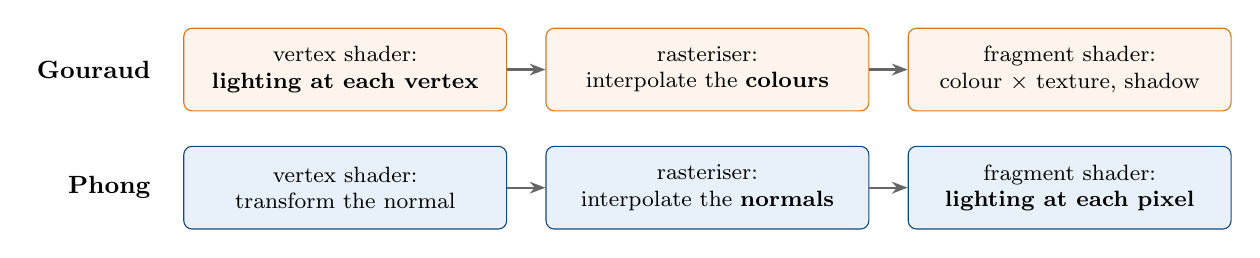
\begin{tikzpicture}[
  bx/.style={draw, rounded corners=3pt, minimum width=4.1cm, minimum height=1.05cm,
             align=center, font=\footnotesize},
  g/.style={bx, draw=elec, fill=elec!8}, p/.style={bx, draw=accent, fill=accentlight},
  arr/.style={-{Stealth[length=2mm]}, thick, black!60}]
\node[font=\small\bfseries, anchor=east] at (-2.35,0) {Gouraud};
\node[g] (g1) at (0,0) {vertex shader:\\ \textbf{lighting at each vertex}};
\node[g] (g2) at (4.6,0) {rasteriser:\\ interpolate the \textbf{colours}};
\node[g] (g3) at (9.2,0) {fragment shader:\\ colour $\times$ texture, shadow};
\node[font=\small\bfseries, anchor=east] at (-2.35,-1.5) {Phong};
\node[p] (p1) at (0,-1.5) {vertex shader:\\ transform the normal};
\node[p] (p2) at (4.6,-1.5) {rasteriser:\\ interpolate the \textbf{normals}};
\node[p] (p3) at (9.2,-1.5) {fragment shader:\\ \textbf{lighting at each pixel}};
\draw[arr] (g1)--(g2); \draw[arr] (g2)--(g3);
\draw[arr] (p1)--(p2); \draw[arr] (p2)--(p3);
\end{tikzpicture}
\caption{Where the lighting is evaluated in Gouraud and Phong shading.}
\label{fig:shadingpipe}
\end{figure}

\textbf{Gouraud shading}~\cite{gouraud} evaluates the lighting equation only at the
three vertices of a triangle and lets the rasteriser blend the resulting colours.
For a pixel with barycentric weights $\lambda_0+\lambda_1+\lambda_2 = 1$,
\begin{equation}
I(\vect{x}) = \lambda_0 I_0 + \lambda_1 I_1 + \lambda_2 I_2 .
\end{equation}
It is cheap, but a highlight that falls between the vertices of a large triangle is
lost, because no vertex sees it. In the project, \code{gouraud.vert} computes the
ambient and point-light colour, the sun's diffuse colour and the sun's specular
colour per vertex. \code{gouraud.frag} only multiplies them by the texture and applies
the shadow per pixel, so shadows stay sharp while the lighting itself stays per vertex.

\textbf{Phong shading}~\cite{phong} interpolates the \emph{normal} instead and
evaluates the full lighting equation for every pixel:
\begin{equation}
\vect{N}(\vect{x}) = \text{normalize}\!\left(\lambda_0\vect{N}_0 + \lambda_1\vect{N}_1 + \lambda_2\vect{N}_2\right),\qquad
I(\vect{x}) = \text{shade}\big(\vect{N}(\vect{x}),\,\vect{x}\big).
\end{equation}
Highlights are sharp and correctly placed even on big triangles. The project
implements this in \code{lit.vert} and \code{lit.frag}. Both paths call the same
lighting terms from \code{common.glsl}, so the comparison is fair: the only difference
is \emph{where} the equation is evaluated.

\begin{figure}[!htbp]
\centering
\begin{subfigure}[t]{0.49\textwidth}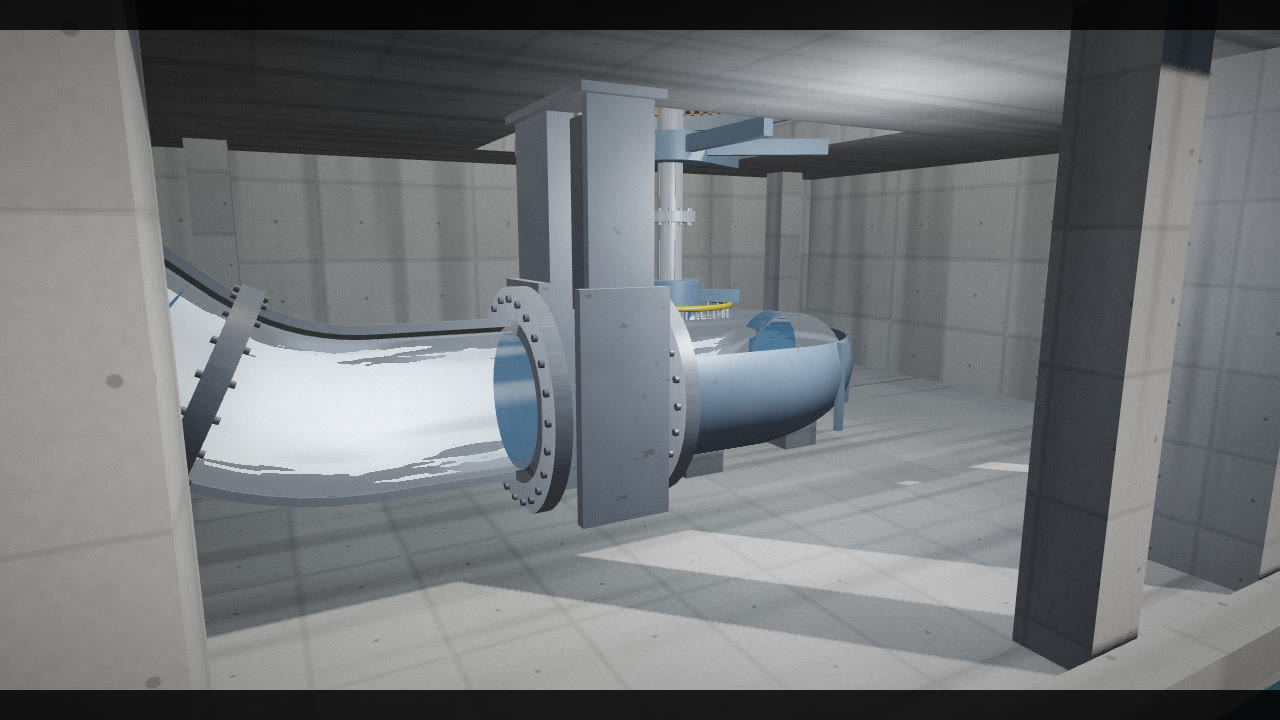
\includegraphics[width=\linewidth]{phong_valve.jpg}\caption{Phong: the sun's highlight on the large ceiling panels and the bright reflection on the pipe are clear.}\end{subfigure}\hfill
\begin{subfigure}[t]{0.49\textwidth}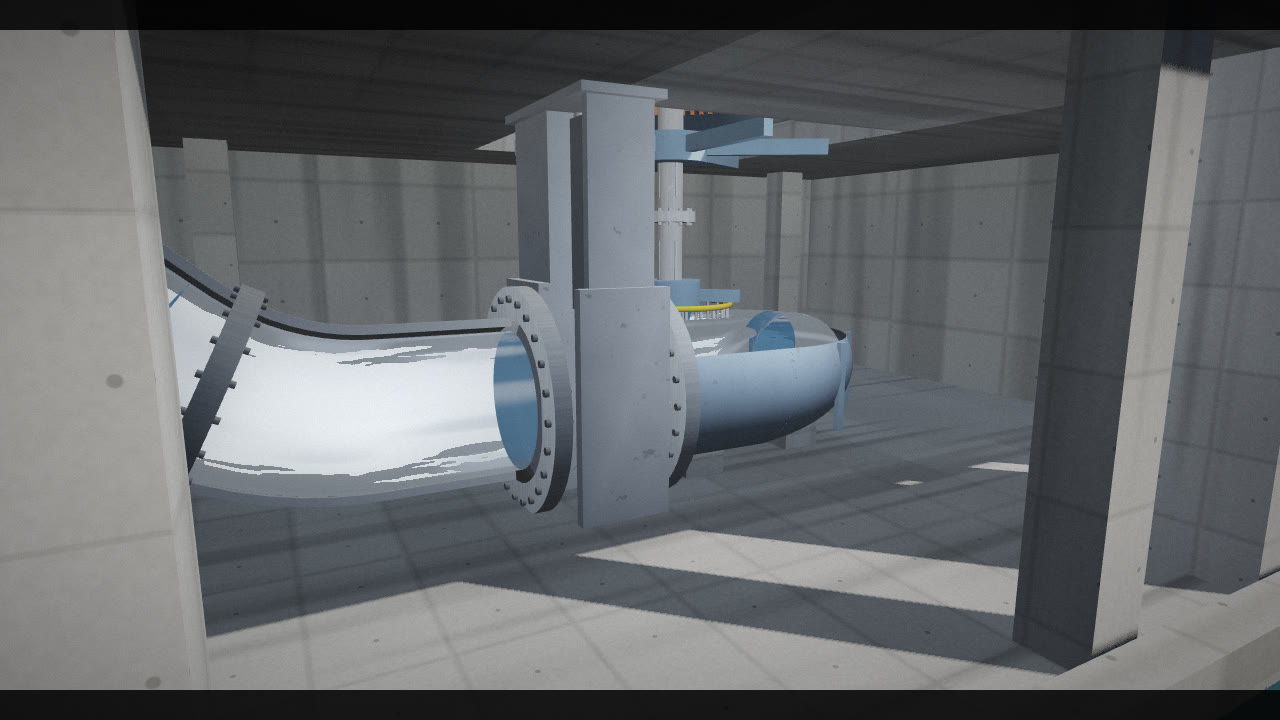
\includegraphics[width=\linewidth]{gouraud_valve.jpg}\caption{Gouraud: the same view; the highlight between the vertices of the ceiling is lost.}\end{subfigure}
\caption{The same frame of scene 6 rendered with Phong and with Gouraud shading.}
\label{fig:gouraudphong}
\end{figure}

\key{G} cycles through three modes: \emph{Mixed} (the default: the large, smooth
terrain uses Gouraud, everything else uses Phong), \emph{all Phong} and \emph{all
Gouraud}. The Renderer picks the shader program for each draw call according to the
mode and a per-material preference.

\section{Shadow Mapping}
\label{sec:shadow}

Shadows use the two-pass shadow-map method~\cite{williams}. In the first pass the
scene is drawn from the sun's point of view into a 2048$\times$2048 depth texture.
The light's view matrix looks from $\vect{c} + 2r\,\vect{L}$ towards the centre
$\vect{c}$ of the area of interest, and an orthographic projection covers a square of
half-size $r$. Each scene chooses $\vect{c}$ and $r$, so the resolution is spent where
the camera is looking. In the second pass, every pixel is transformed into the same
light space:
\begin{equation}
\vect{p}_L = \mat{P}_L\,\mat{V}_L\,(\vect{x} + \delta\,\vect{N}),\qquad
(u, v, z) = \tfrac12\,\vect{p}_L.xyz/\vect{p}_L.w + \tfrac12 .
\end{equation}
The point is in shadow if something nearer to the sun was stored in the depth map at
$(u,v)$. Moving the point a little along its normal ($\delta$, three texels) and a small
depth bias $b$ prevent ``shadow acne'', the stripes that appear when a surface shadows
itself. Polygon offset is also enabled in the shadow pass. Hard shadow edges are
softened with $3\times3$ percentage-closer filtering~\cite{reeves87}:
\begin{equation}
S = \frac19\sum_{i=-1}^{1}\sum_{j=-1}^{1}
\Big[\,z - b \le D\big(u + 1.25\,i\,\Delta,\ v + 1.25\,j\,\Delta\big)\Big],
\end{equation}
where $D$ is the stored depth, $\Delta$ the size of one texel and $[\cdot]$ is one when
the condition holds and zero otherwise.

\begin{figure}[!htbp]
\centering
\begin{subfigure}[t]{0.49\textwidth}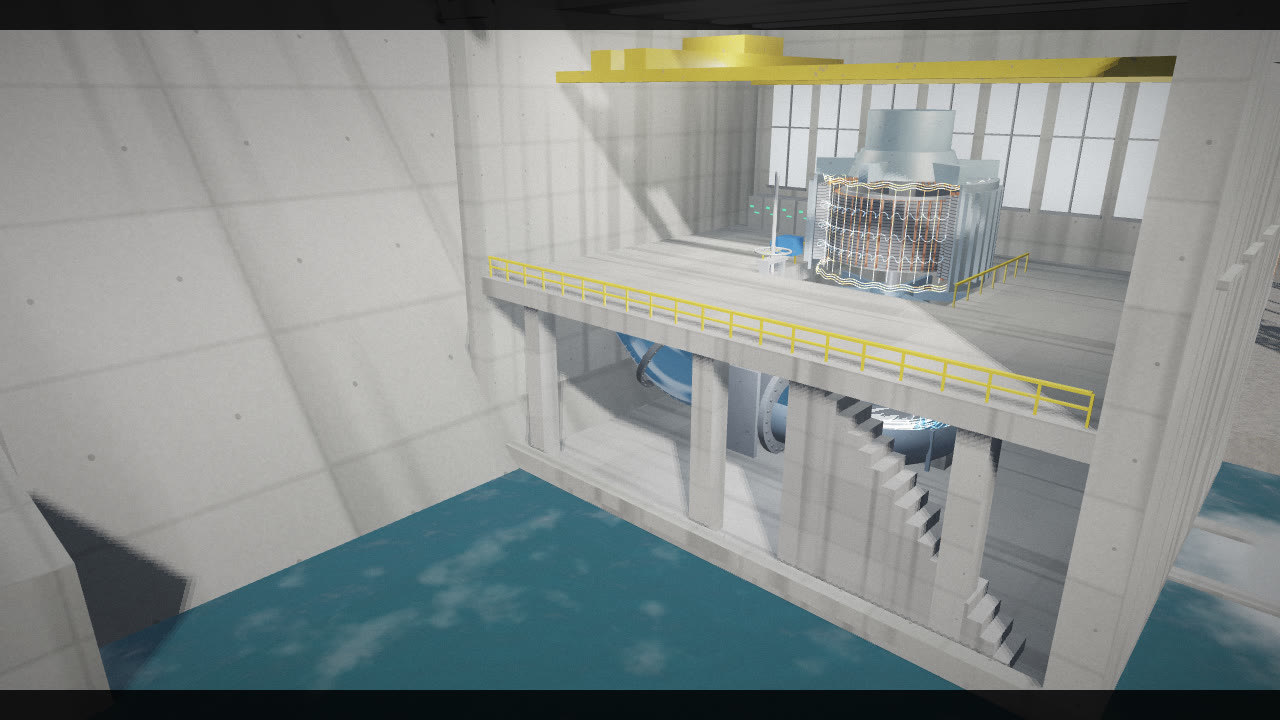
\includegraphics[width=\linewidth]{shadow_on.jpg}\caption{Shadows on: the dam, piers and railings cast soft shadows.}\end{subfigure}\hfill
\begin{subfigure}[t]{0.49\textwidth}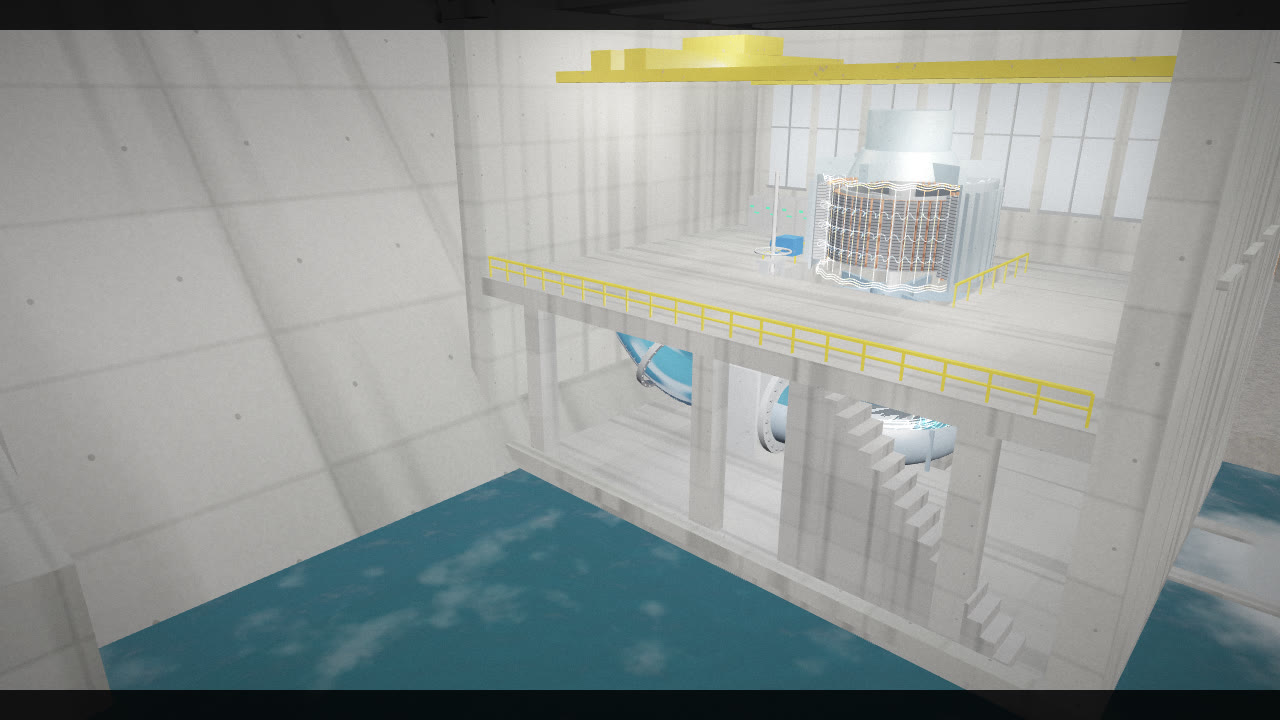
\includegraphics[width=\linewidth]{shadow_off.jpg}\caption{Shadows off (\key{L}): the scene looks flat.}\end{subfigure}
\caption{Effect of shadow mapping on the preview scene.}
\label{fig:shadow}
\end{figure}

\section{Procedural Textures}

Every surface pattern is calculated in the fragment shader (\code{materials.glsl}),
so no image files are needed. The basis is \emph{value noise}: random values at the
corners of a grid, blended with the smooth curve $s(t) = 3t^2-2t^3$. Several octaves
are added to form fractal noise,
\begin{equation}
\text{fbm}(\vect{p}) = \sum_{i=0}^{3} \frac{1}{2^{i+1}}\,\text{noise}\!\left(2^{i}\vect{p}\right),
\end{equation}
which gives detail at several scales, like real stone. The random values come from
Hoskins' arithmetic hash~\cite{hoskins}, which behaves the same on every GPU.
Table~\ref{tab:patterns} lists the 15 patterns.

\begin{table}[!htbp]
\centering
\caption{Procedural material patterns.}
\label{tab:patterns}
\begin{tabularx}{\textwidth}{@{}L{2.4cm}YL{2.4cm}Y@{}}
\toprule
\textbf{Pattern} & \textbf{Idea} & \textbf{Pattern} & \textbf{Idea} \\
\midrule
Concrete & formwork panels, tie holes, stains & Copper & warm metal with wire lines \\
Steel & brushed noise, high specular & Hologram & glowing grid lines \\
Paint & smooth colour with slight wear & Leaf & vein pattern, alpha cut-out \\
Bark & stretched noise along the log & Light beam & soft additive shafts under water \\
Terrain & rock, grass and silt by height and slope & Rock & strong fbm, dark cracks \\
Soil & dark wet noise & Plastic & shiny, coloured \\
Tiles & floor tiles with grout lines & Flow & moving glowing pulses \\
Grating & wire mesh cut out with \code{discard} & & \\
\bottomrule
\end{tabularx}
\end{table}

The terrain is a good example of combining rules. Its colour is chosen from slope and
height: steep parts become rock, flat parts above the water become grass, and parts
below the water line become wet silt, with fbm noise breaking up the borders.

\section{Water Rendering}

Water appears in many forms: the reservoir and river, thin sheets on the spillway,
the jet in the conduit, the tube of water in the penstock, the swirl in the spiral
casing, and the cut faces of water in the cut-away views. One shader pair,
\code{water.vert} and \code{water.frag}, handles all of them through a \emph{mode}.

\textbf{Waves.} Vertices on a free surface are lifted by a sum of three sine waves
that drift with the current $u$:
\begin{multline}
h(x,z,t) = A\big[0.5\sin(f q_x + 1.3t) + 0.3\sin(1.4 f q_z - 1.1t + 0.5 f q_x)\\
 + 0.2\sin(2.3 f (q_x+q_z) + 2.1t)\big],\qquad \vect{q} = (x - ut,\ z).
\end{multline}
In the fragment shader the same function is differentiated numerically to get a
detailed normal, $\vect{N} = \text{normalize}(\vect{N}_0 - \nabla h)$, which is a form
of bump mapping.

\textbf{Reflection and colour.} The final colour mixes the water's body colour with
the reflected sky according to the Fresnel term (Schlick, $F_0 = 0.02$ for water),
plus a sharp sun glitter $\max(\vect{N}\cdot\vect{H},0)^{900}$ and foam where the water
is fast.

\textbf{Snell's window.} When the camera is under water and looks up, the shader
refracts the view ray out of the water with $n = 1.33$. Inside a cone of about
$48.8^\circ$ (the critical angle, $\arcsin(1/1.33)$) the sky is visible; outside it the ray is totally reflected and the surface
looks like a mirror, which is what divers see.

\textbf{Moving water fronts.} The water in the conduit and penstock has a front that
moves with the simulation. Fragments beyond the front are discarded, and in the
penstock the vertex shader pulls the vertices just beyond the front towards the pipe
axis using $r' = r\sqrt{1-k^2}$, which gives the advancing water a rounded nose.

\section{Ray Tracing}
\label{sec:rt}

Scene 5 is drawn by a completely different method. Instead of rasterising triangles,
one full-screen triangle is drawn and the fragment shader \code{raytrace.frag} traces
a ray for every pixel through a scene described by exact mathematics: a glass penstock
with steel sleeves, flanges, concrete supports, a glossy floor and a back wall. The
algorithm is Whitted-style recursive ray tracing~\cite{whitted}, unrolled to a fixed
depth because GLSL does not allow recursion. Figure~\ref{fig:rtdiagram} shows the rays
involved.

\begin{figure}[htbp]
\centering
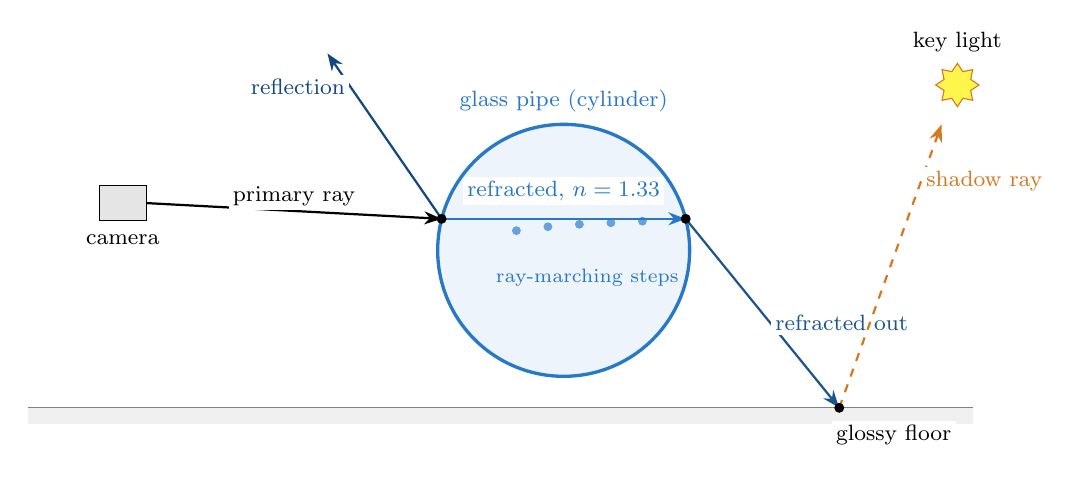
\begin{tikzpicture}[scale=1.0,
  ray/.style={-{Stealth[length=2.2mm]}, thick},
  lbl/.style={font=\footnotesize, fill=white, inner sep=1.5pt}]
\fill[black!6] (-1.2,-2.2) rectangle (10.8,-2.0);
\draw[black!50] (-1.2,-2.0) -- (10.8,-2.0);
\node[lbl, anchor=west] at (9.0,-2.35) {glossy floor};
\draw[water, line width=1.2pt, fill=water!8] (5.6,0) circle (1.6);
\node[lbl, text=water] at (5.6,1.9) {glass pipe (cylinder)};
\foreach \x/\y in {5.0/0.25, 5.4/0.3, 5.8/0.33, 6.2/0.35, 6.6/0.37}
  \fill[water!70] (\x,\y) circle (1.6pt);
\node[font=\scriptsize, text=water] at (5.9,-0.35) {ray-marching steps};
\node[draw, fill=black!10, minimum width=0.6cm, minimum height=0.45cm] (cam) at (0,0.6) {};
\node[lbl, anchor=north] at (0,0.25) {camera};
\coordinate (P1) at (4.05,0.4);
\draw[ray, black] (0.3,0.6) -- (P1) node[lbl, midway, above] {primary ray};
\draw[ray, accent] (P1) -- (2.6,2.5) node[lbl, pos=0.8, left] {reflection};
\coordinate (P2) at (7.15,0.4);
\draw[ray, water] (P1) -- (P2);
\node[lbl, text=water] at (5.6,0.75) {refracted, $n=1.33$};
\draw[ray, water!70!black] (P2) -- (9.1,-2.0) node[lbl, pos=0.55, right] {refracted out};
\coordinate (F) at (9.1,-2.0);
\draw[ray, elec, dashed] (F) -- (10.4,1.6) node[lbl, pos=0.8, right] {shadow ray};
\node[star, star points=8, fill=yellow!70, draw=elec, minimum size=0.55cm] at (10.6,2.1) {};
\node[lbl] at (10.6,2.65) {key light};
\fill (P1) circle (1.8pt); \fill (P2) circle (1.8pt); \fill (F) circle (1.8pt);
\end{tikzpicture}
\caption{Rays traced for one pixel that hits the glass pipe.}
\label{fig:rtdiagram}
\end{figure}

\subsection{Primary rays}

For a pixel at normalised device coordinates $(x_n, y_n)\in[-1,1]^2$, the ray starts
at the camera $\vect{o}$ and points along
\begin{equation}
\vect{d} = \text{normalize}\!\left(\vect{F} + x_n\tan\tfrac{\varphi}{2}\,a\,\vect{R} + y_n\tan\tfrac{\varphi}{2}\,\vect{U}\right),
\end{equation}
where $\vect{F}$, $\vect{R}$, $\vect{U}$ are the camera's forward, right and up vectors.
The ray is $\vect{r}(t) = \vect{o} + t\,\vect{d}$, and the task is to find the smallest
positive $t$ at which it hits something.

\subsection{Ray--surface intersections}

\textbf{Infinite cylinder (the pipe).} The pipe has axis point $\vect{A}$, unit
direction $\vect{D}$ and radius $r$. Removing the components along the axis,
$\vect{d}_\perp = \vect{d} - (\vect{d}\cdot\vect{D})\vect{D}$ and
$\vect{o}_\perp = (\vect{o}-\vect{A}) - ((\vect{o}-\vect{A})\cdot\vect{D})\vect{D}$,
the hit condition $\lVert\vect{o}_\perp + t\,\vect{d}_\perp\rVert = r$ becomes the
quadratic
\begin{equation}
a\,t^2 + 2b\,t + c = 0,\qquad a = \vect{d}_\perp\cdot\vect{d}_\perp,\quad
b = \vect{o}_\perp\cdot\vect{d}_\perp,\quad c = \vect{o}_\perp\cdot\vect{o}_\perp - r^2,
\end{equation}
\begin{equation}
t_{1,2} = \frac{-b \mp \sqrt{b^2 - a c}}{a}.
\end{equation}
There is no hit when $b^2-ac<0$. The normal at the hit point $\vect{q}$ is the radial
direction, $\text{normalize}\big((\vect{q}-\vect{A}) - ((\vect{q}-\vect{A})\cdot\vect{D})\vect{D}\big)$.
The axial position $s$ decides the material: the pipe repeats every 16\,m, and the
first 11\,m of each period are glass, the rest steel.

\noindent\begin{minipage}{\linewidth}
\begin{lstlisting}
vec2 cylinder(vec3 ro, vec3 rd, float r) {        // raytrace.frag
    vec3 oc  = ro - uPipeA;
    vec3 rdp = rd - uPipeDir * dot(rd, uPipeDir);  // remove the axial parts
    vec3 ocp = oc - uPipeDir * dot(oc, uPipeDir);
    float a = dot(rdp, rdp), b = dot(ocp, rdp), c = dot(ocp, ocp) - r * r;
    float h = b * b - a * c;                       // discriminant
    if (h < 0.0) return vec2(-1.0);                // miss
    h = sqrt(h);
    return vec2((-b - h) / a, (-b + h) / a);       // entry and exit
}
\end{lstlisting}
\end{minipage}

\textbf{Capped cylinders (flanges and bands)} use Quilez's closed-form
intersection~\cite{iq}, which tests the side and both end caps in one function.

\textbf{Boxes (supports)} use the slab method: for each axis the ray enters and leaves
the slab between two planes at
$t_0 = (\vect{b}_{\min}-\vect{o})/\vect{d}$ and $t_1 = (\vect{b}_{\max}-\vect{o})/\vect{d}$
(component-wise). The box is hit if
$t_{\text{near}} = \max(\min(t_0,t_1)) \le t_{\text{far}} = \min(\max(t_0,t_1))$ and
$t_{\text{far}} > 0$.

\textbf{Planes (floor and wall)}: for the floor $y=0$, $t = -o_y/d_y$ when $d_y<0$.

\subsection{Shading, shadows, reflection and refraction}

\textbf{Shadow rays.} From a hit point a second ray is sent towards the key light.
If it hits steel or concrete, the point is in shadow (only 12\,\% of the light
remains). If it hits glass, blue-tinted light passes through, so the floor under the
pipe receives a coloured shadow.

\textbf{Reflection.} The glossy floor, the glass and the steel send a reflection ray
in the mirror direction
\begin{equation}
\vect{r} = \vect{d} - 2(\vect{d}\cdot\vect{N})\,\vect{N},
\end{equation}
weighted by the Fresnel term. For glass, $F = 0.04 + 0.96\,(1-\cos\theta_i)^5$.

\textbf{Refraction.} At the glass the ray bends into the water according to Snell's
law $n_1\sin\theta_1 = n_2\sin\theta_2$. In vector form, with
$\eta = n_1/n_2 = 1/1.33$ and $\cos\theta_i = -\vect{N}\cdot\vect{d}$,
\begin{equation}
\vect{t} = \eta\,\vect{d} + \left(\eta\cos\theta_i - \sqrt{1-\eta^2(1-\cos^2\theta_i)}\right)\vect{N}.
\end{equation}
When the ray leaves the water the ratio is inverted. If the value under the square
root is negative, the light cannot leave the water (total internal reflection), and
the ray is reflected instead.

\textbf{Volume ray marching.} The water does not have a single surface; it is a volume
full of glowing streaks. Between the entry and exit points the ray is split into 36
steps. At each step the shader evaluates a density $\rho(\vect{p})$ built from noise
that moves along the pipe at the flow speed, adds the emitted light and reduces the
transmittance $T$ with the Beer--Lambert law:
\begin{equation}
L \mathrel{+}= \vect{e}(\vect{p})\,\rho(\vect{p})\,\Delta t\,T,\qquad
T \leftarrow T\,\exp\!\big(-\Delta t\,(0.05 + 0.12\,\rho(\vect{p}))\big).
\end{equation}
The start of each march is jittered by a random fraction of a step per pixel, which
hides banding. The glass colour is finally
$\vect{C} = \text{mix}(\vect{C}_{\text{transmitted}}, \vect{C}_{\text{reflected}}, F)$.

\subsection{Interaction with the ray tracer}

\key{UP} and \key{DOWN} change the head $H$ in steps of 10\,m. The C++ side computes
the jet speed $v = \sqrt{2gH}$, the flow $Q = 180\sqrt{H/53}$ and the power from
Equation~\eqref{eq:power}, and passes the speed to the shader, so the glowing streaks
visibly race faster or slower. A moving scan ring and the hologram floor grid give the
scene a futuristic, diagram-like look.

\section{Animation and Physics}

\subsection{Time step and speed control}

All motion is driven by the frame time. Every scene update receives
$\Delta t_{\text{scene}} = \Delta t \times s$ with $s\in\{0.25, 0.5, 1, 2\}$, so the
whole world (water, machines, particles, cameras) can be watched in slow or fast
motion. The water is additionally shown at 0.55--0.6 of its real speed so the eye can
follow it.

\subsection{Free-falling water}

The spillway sheets and the penstock water are modelled as fronts that travel along a
path. The speed at a point depends on how far the water has dropped, from energy
conservation:
\begin{equation}
v(s) = \sqrt{v_0^2 + 2\,g\,\Delta h(s)},\qquad s \leftarrow s + v(s)\,\Delta t ,
\end{equation}
with $v_0 = 2$\,m/s on the spillway and $6$\,m/s in the penstock. The water therefore
starts slowly and accelerates downhill. When a gate closes, the tail of the water runs
down the same way, so the chute drains instead of the water simply vanishing.

Under the intake gate the water jets out with Torricelli's speed~\cite{white},
\begin{equation}
v_{\text{jet}} = \sqrt{2\,g\,h} = \sqrt{2 \times 9.81 \times 17} \approx 18.3\ \text{m/s},
\end{equation}
where $h$ is the depth of the opening below the reservoir surface. The conduit's water
surface is rebuilt every frame as a height profile with a bulge behind the gate, a
rounded front and a rising level.

\subsection{Machines with inertia}

Real machines do not jump to a new state. Gates, the valve, the guide vanes, the field
current and the breaker move at limited rates:
\begin{equation}
x \leftarrow x + \text{clamp}\big(x_{\text{target}} - x,\ -r\,\Delta t,\ r\,\Delta t\big).
\end{equation}
The runner speed follows the flow like a first-order system with a time constant of
about two seconds:
\begin{equation}
\omega \leftarrow \omega + \big(\omega_{\text{target}} - \omega\big)\,\min(0.45\,\Delta t, 1),
\qquad \omega_{\text{target}} = \Omega_v \min(1, 1.25\,q).
\end{equation}
This is why the turbine keeps turning for a short time after the water stops.

\subsection{Floating debris}

Each piece of trash is simulated in the local flow frame. The current drags it along
$x$, a spring--damper holds it at its floating depth, and it bobs gently:
\begin{align}
v_x &\leftarrow v_x + (u - v_x)\min(1.5\,\Delta t, 1), \\
y_{\text{target}} &= y_{\text{float}} + 0.12\sin(1.6\,t + \phi), \\
v_y &\leftarrow v_y + \big(2.5\,(y_{\text{target}} - y) - 1.8\,v_y\big)\Delta t, \\
\vect{x} &\leftarrow \vect{x} + \vect{v}\,\Delta t .
\end{align}
At the trash rack a piece larger than the 0.56\,m gap stops, throws a splash of
particles and settles against the bars; small leaves squeeze through and are drawn
down into the intake.

\subsection{Particle systems}

Spray, mist, outflow foam, splashes, gate spray and under-water dust are particle
systems~\cite{reeves83}. Each particle has a position, velocity, size, colour and
lifetime, and is integrated with explicit Euler steps including gravity and drag:
\begin{equation}
v_y \leftarrow v_y + g\,\Delta t,\qquad
\vect{v} \leftarrow \frac{\vect{v}}{1 + k_d\,\Delta t},\qquad
\vect{x} \leftarrow \vect{x} + \vect{v}\,\Delta t,\qquad
\text{size} \leftarrow \text{size} + \gamma\,\Delta t .
\end{equation}
The opacity fades in quickly and out slowly, $\alpha = \alpha_0\min(1, 8k)(1-k)$ with
$k = \text{age}/\text{lifetime}$. Each particle is drawn as a quad that always faces
the camera (a billboard), built from the camera's right and up vectors
$\vect{x}\pm s\vect{R}\pm s\vect{U}$. Dead particles are removed by swapping them with
the last element, which costs constant time.

\subsection{Glowing flow lines}

The invisible things in the plant (the paths of the water through the turbine, the
magnetic field and the electric current) are shown with \emph{flow lines}: thin tubes
along a path whose texture coordinate $s$ is the distance along the path. The shader
draws bright pulses that move along the line:
\begin{equation}
\phi = \text{fract}\big(\sigma s - \sigma v t\big),\qquad
\text{pulse} = \text{smoothstep}(0, 0.08, \phi)\,\big(1-\text{smoothstep}(0.08, 0.6, \phi)\big),
\end{equation}
where $\sigma$ is the number of pulses per metre and $v$ their speed. A \emph{front}
value hides everything beyond the point the water or the energy has reached, and the
tip of the front glows brighter. The same technique shows 24 water streamlines through
the turbine, the field lines around the rotor poles, the orange three-phase current in
the stator coils and bus ducts, and the energy travelling 640\,m along the power line.

\subsection{Three-phase oscilloscope}

The generator scene draws three sine waves, each shifted by $120^\circ$:
\begin{equation}
y_p(u) = A\,\sin\!\left(2\pi(c\,u - k\,t) - \frac{2\pi p}{3}\right),\qquad p = 0, 1, 2,
\end{equation}
where the amplitude $A$ is proportional to the terminal voltage. The waves therefore
grow from nothing when the rotor is excited.

\section{Post-Processing and Transitions}

The 3D image is first rendered into a texture. Three small shaders then give it a
cinematic finish (\code{render/PostFX.cpp}):

\begin{enumerate}
  \item \textbf{Bright pass} at a quarter of the screen size keeps only the bright
        parts, using the luminance $Y = 0.2126R + 0.7152G + 0.0722B$ and a soft threshold
        $k = \text{smoothstep}(0.78, 1, Y)$.
  \item \textbf{Gaussian blur}, done separably: first horizontally, then vertically.
        A $9$-tap filter with weights $w = (0.227, 0.195, 0.122, 0.054, 0.016)$ is
        applied in each direction~\cite{learnopengl}. Two one-dimensional passes cost
        $2\times9$ samples instead of $81$.
  \item \textbf{Composite}: the blurred glow $\vect{g}$ is added to the image
        (\emph{bloom}), the corners are darkened with $1 - 0.76\,\lVert\vect{d}\rVert^2$
        (\emph{vignette}), and a little animated noise is added (\emph{film grain}).
\end{enumerate}

The whole pass costs about one millisecond and can be switched off with \key{V}
(Figure~\ref{fig:bloom}).

\begin{figure}[!htbp]
\centering
\begin{subfigure}[t]{0.49\textwidth}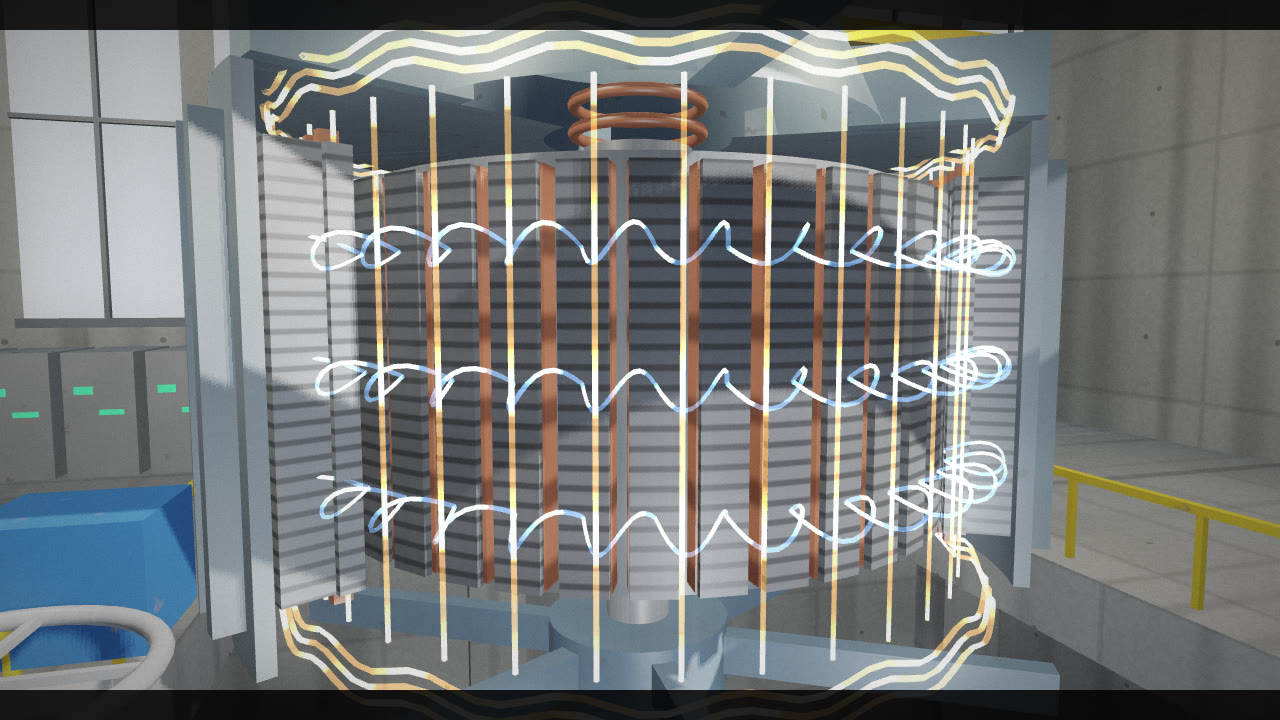
\includegraphics[width=\linewidth]{bloom_on.jpg}\caption{Bloom on: the current and field lines glow.}\end{subfigure}\hfill
\begin{subfigure}[t]{0.49\textwidth}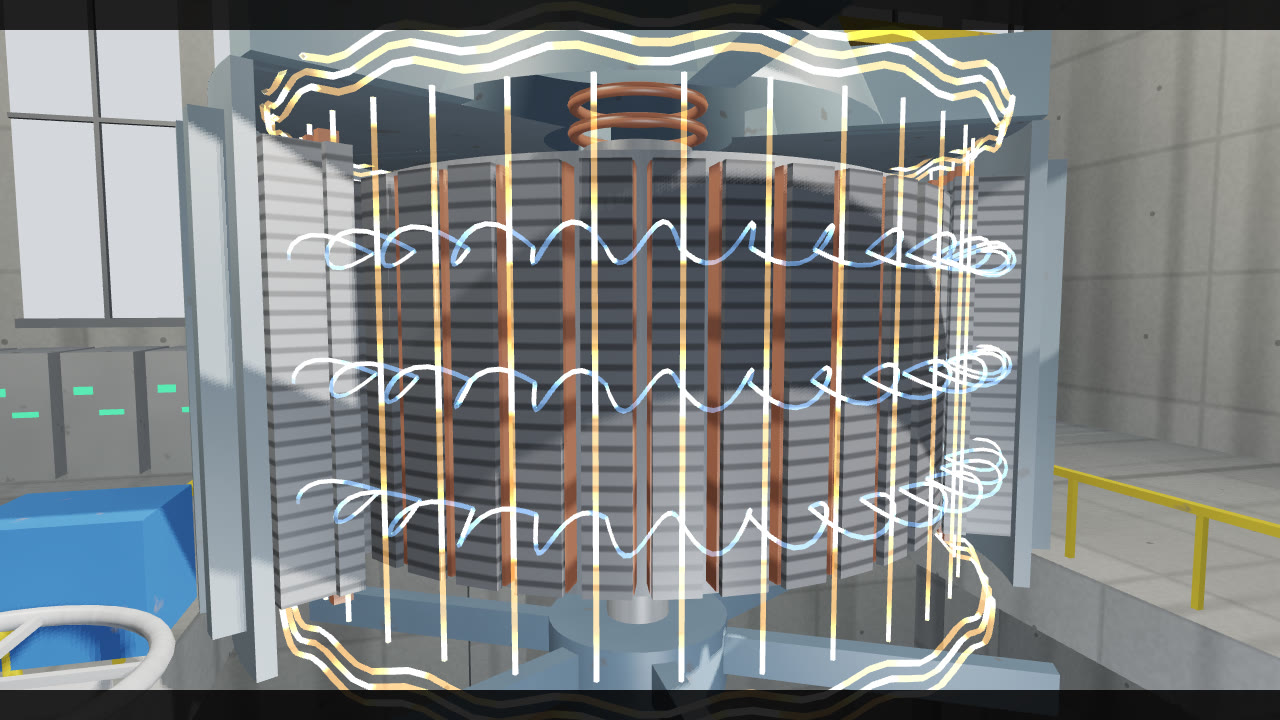
\includegraphics[width=\linewidth]{bloom_off.jpg}\caption{Bloom off (\key{V}).}\end{subfigure}
\caption{Post-processing on the generator scene.}
\label{fig:bloom}
\end{figure}

\textbf{Cross-dissolve.} When the render style changes completely, for instance from
the raster world to the ray tracer, the last frame is kept in a texture
(\code{render/FrameCapture.cpp}) and blended over the new scene with an opacity that
falls from one to zero over 1.1\,s along the smooth curve $\alpha = x^2(3-2x)$.
Elsewhere the camera simply flies on.

\section{User Interface and Text}

The HUD (\code{ui/Ui.cpp}) is drawn in pixel coordinates with an orthographic
mapping: a pixel $(x,y)$ goes to $(2x/W - 1,\ 1 - 2y/H)$ in clip space. Text uses a
hand-made font (\code{ui/Font.cpp}): each of the 63 glyphs (capital letters, digits and
punctuation) is written in the source as seven strings of five characters, where
\texttt{\#} marks a lit pixel. At start-up the
glyphs are packed into a small texture with $6\times8$ cells and sampled with nearest
filtering, so the letters stay crisp at any integer scale. Text positions are snapped
to whole pixels so that a glyph never samples its neighbour in the atlas.

Labels that point at 3D parts use the same projection as the renderer: the part's
world position is multiplied by $\mat{P}\mat{V}$, divided by $w$, and mapped to the
screen. A leader line then joins the point to the label, and labels are pushed out of
the title and telemetry panels if they would overlap them.

\section{Interaction}

Interaction happens on three levels. \textbf{Scene buttons} at the bottom of the
screen drive the story; each has a keyboard shortcut shown under it. A button whose
cause has not happened yet is drawn in grey with a hint (``open the gate first'',
``wait, the casing is filling''), which teaches the order of operation without
any extra text. \textbf{Global controls} work in every scene (Table~\ref{tab:keys}).
\textbf{The mouse} orbits, pans and zooms the camera on top of the director's camera.

\begin{table}[!htbp]
\centering
\caption{Global controls.}
\label{tab:keys}
\small
\begin{tabularx}{\textwidth}{@{}L{3.3cm}YL{2.6cm}Y@{}}
\toprule
\textbf{Input} & \textbf{Action} & \textbf{Input} & \textbf{Action} \\
\midrule
Left mouse drag & Orbit around the target & \key{L} & Shadows on and off \\
Right drag, \key{W}\key{A}\key{S}\key{D}\key{Q}\key{E} & Move (pan) the camera & \key{V} & Bloom, vignette and grain on and off \\
Mouse wheel & Zoom & \key{H} & Hide or show the HUD \\
\key{C} & Back to the director's camera & \key{P} & Automatic play-through of the whole story (about three minutes) \\
\key{[} \key{]} or buttons & Speed 0.25$\times$, 0.5$\times$, 1$\times$, 2$\times$ & \key{1}--\key{9}, \key{0} & Jump to scenes 1--10 \\
\key{G} & Shading: Mixed, Phong, Gouraud & \key{N}/\key{B}, arrows & Next or previous scene \\
\key{F12} & Save a screenshot as a BMP file & \key{R} & Restart the current scene \\
 & & \key{Esc} & Quit \\
\bottomrule
\end{tabularx}
\end{table}

% =====================================================================
%  CHAPTER 5  OBJECTS
% =====================================================================
\chapter{Objects of the Scene}
\label{ch:objects}

Each object has its own source file in \code{src/objects/} and is built entirely from
the primitives of Section~\ref{sec:geometry}. The world uses metres, with $x$ along the
dam crest, $y$ up and $z$ downstream. Table~\ref{tab:objlist} gives an overview, and
the sections that follow describe how each object is built and how it moves.

\begin{longtable}{@{}L{3.0cm}L{4.15cm}L{4.0cm}L{3.2cm}@{}}
\caption{Objects in the scene.}\label{tab:objlist}\\
\toprule
\textbf{Object} & \textbf{File} & \textbf{Built from} & \textbf{Moving parts} \\
\midrule
\endfirsthead
\toprule
\textbf{Object} & \textbf{File} & \textbf{Built from} & \textbf{Moving parts} \\
\midrule
\endhead
\bottomrule
\endfoot
Valley terrain & \code{Terrain.cpp} & 260$\times$260 height-field grid from fbm noise & -- \\
Boulders & \code{Rocks.cpp} & spheres displaced by noise & -- \\
Gravity dam & \code{Dam.cpp} & extruded profile, piers, crest, gantry crane & 3 spillway gates, cut block \\
Spillway water & \code{SpillwayWater.cpp} & sheets following the chute profile & free-falling fronts \\
Intake structure & \code{IntakeStructure.cpp} & boxes, deck, rake motors & -- \\
Trash rack & \code{TrashRack.cpp} & flat bars, beams, brackets & -- \\
Floating debris & \code{Debris.cpp} & branch, logs, plastic, straw, leaves & 29 pieces per wave \\
Intake gate & \code{IntakeGate.cpp} & leaf, ribs, cylinders, rods & gate and 2 rods \\
Penstock & \code{CutawayPipe.cpp} & swept tube with cut, rings, bolts & water front \\
Powerhouse & \code{Powerhouse.cpp} & walls, floors, windows, railings, crane & shaft \\
Main inlet valve & \code{MainInletValve.cpp} & flanges, body, bonnet, gate, wheel & gate, stem, wheel \\
Francis turbine & \code{TurbineUnit.cpp} & spiral sweep, vanes, runner, draft tube & 24 vanes, ring, runner \\
Generator & \code{Generator.cpp} & stator ring, 72 slots, rotor, 40 poles & rotor \\
Transformer & \code{Transformer.cpp} & tank, radiators, fans, bushings, ducts & 4 fans \\
Switchyard & \code{Switchyard.cpp} & gantries, breakers, CTs, arresters & status lamps \\
Power line & \code{TransmissionLine.cpp} & 10 lattice towers, sagging wires & energy glow \\
Flow lines & \code{FlowLines.cpp} & thin tubes along paths & moving pulses \\
Particles & \code{ParticleSystem.cpp} & camera-facing quads & 6 systems \\
\end{longtable}

\section{Terrain, Reservoir and River}

The valley is a height function $h(x,z)$ evaluated on the CPU at 260$\times$260 points.
It combines a river channel, the reservoir bed upstream, mountain sides that rise away
from the river and fbm noise for natural irregularity. Normals are taken from the
gradient of $h$. The terrain is the largest and smoothest object, so in Mixed mode it
uses Gouraud shading, which is a sensible use of the cheaper method. The reservoir
(level 56\,m) and the river (level 3\,m) are large water grids, and boulders are
spheres pushed in and out by noise with a flattened bottom.

\section{Dam and Spillway}

The concrete gravity dam is 300\,m long with its crest at 63\,m. Its cross-section is
a 2D profile, vertical on the upstream face and sloping on the downstream face,
extruded along the crest. In the middle, three 11\,m spillway bays separated by 4\,m
piers carry vertical-lift gates that translate up by 9.5\,m. The power waterway
passes through the dam at $x = 58$\,m: an intake mouth in the upstream face, an
11$\times$10\,m conduit, a vertical slot for the intake gate and a bulkhead where the
penstock starts. The conduit itself is not a hole cut out of a solid; it is the gap
left between four extruded solid pieces. The section between $x = 24.5$ and $52.5$\,m
is a separate ``cut block'' that lifts away for the cut-away views.

\section{Intake Structure, Trash Rack and Debris}

In front of the intake a concrete structure with side piers and a top deck holds a cage
of trash-rack panels. Each panel is a row of flat steel bars 0.56\,m apart between a top
and a bottom beam. The near half of the structure forms a separate group that is
hidden in the cut-away view so the cage can be seen from the side. Debris pieces are
small meshes (a forked branch, logs, crumpled plastic, straw and leaves) drawn with bark,
plastic and leaf patterns; one wave contains 29 pieces, and \key{T} sends another.

\section{Intake Gate and Penstock}

The intake gate is a steel leaf with ribs, lifted by two hydraulic cylinders standing on
the dam crest. The penstock is a 4\,m diameter steel pipe about 58\,m long that drops
33\,m from the bulkhead to the powerhouse. It is a circle swept along a path with
rounded bends; only part of its circumference is kept, so it is open on the camera side.
Stiffener rings with bolts go round the full pipe. The removed part can be shown as a
glowing X-ray grid, and the water inside is a separate tube whose front moves.

\section{Powerhouse}

The powerhouse stands at the foot of the dam and is drawn as a cut-away with its front
wall removed. It has a turbine pit, the main shaft with a guide bearing and a bolted
coupling flange, a generator floor at 14\,m with yellow railings and control cabinets,
large windows, lamps (point lights) and an overhead crane. The penstock ends at the
main inlet valve inside the pit.

\section{Main Inlet Valve}

The valve sits between the penstock and the spiral casing. Two bolted flanges hold a
cast body with a tall bonnet. Inside, a heavy gate slides up by 4.4\,m into the bonnet
when the valve opens, and a hand-wheel on top turns only while the gate is moving. The
body is cut open on the camera side so the gate can be seen.

\section{Francis Turbine}

The turbine (\code{TurbineUnit.cpp}) is the most detailed object. Water enters a
\emph{spiral casing}: a tube swept along a spiral whose radius shrinks as it wraps round,
so that the water keeps the same speed as it is fed inwards. Inside the casing, 12 fixed
\emph{stay vanes} hold the structure together, and 24 movable \emph{guide vanes} control
how much water reaches the runner. The guide vanes turn together through an operating
ring. The \emph{runner} has 15 curved blades built as twisted strips; the water turns
inwards through them and then flows down the \emph{draft tube} cone to the river. The
casing is open on top, and in section view the near half is hidden. For that view a
second set of streamlines is used that keeps only the far half, so the runner stays
visible.

\section{Generator}

The vertical generator stands on the generator floor above the turbine. The
\emph{stator} is a ring of thin steel sheets with 72 slots, each holding a copper coil
that loops round at the top and bottom (end windings). The \emph{rotor} has a hub,
spider arms, a rim and 40 poles, each wrapped in a copper field coil. The housing has a
$120^\circ$ window cut towards the camera. Exciting the rotor makes blue magnetic field
lines appear around the poles; once the rotor spins with a field, orange current pulses
run through the stator coils at a rate set by the frequency.

\section{Bus Ducts and Step-up Transformer}

Three isolated-phase bus ducts carry the generator current out through the wall and
drop onto the low-voltage bushings of the transformer. The transformer has a green
tank, radiator banks, four cooling fans that spin only while there is voltage, a
conservator tank and tall brown high-voltage bushings. The X-ray view makes the tank
transparent and shows the iron core with three legs, each carrying a low-voltage
winding with few turns and a high-voltage winding with many turns. This is the 1\,:\,20
turns ratio that raises 11\,kV to 220\,kV.

\section{Switchyard and Power Line}

The switchyard follows the order in which the power flows: transformer bushings, a
gantry, a disconnector, the circuit breaker, current transformers, surge arresters and
the line gantry. Status lamps on the breakers fade from red (open) to green (closed).
The power line has ten lattice steel towers marching down the valley. Six conductors
in two circuits and an earth wire hang between them; each span is a sagging curve, a
parabola close to the true catenary, $y(x) = y_{\text{lin}}(x) - 4\,s\,u(1-u)$ for a
span parameter $u\in[0,1]$ and sag $s$. When the breaker closes, a glow travels along
the conductors at 140\,m/s and the camera follows it.

\section{Summary of Moving Objects}

Table~\ref{tab:moving} counts everything that moves in the world.

\begin{table}[H]
\centering
\caption{Moving objects in the world.}
\label{tab:moving}
\begin{tabularx}{\textwidth}{@{}L{4.8cm}L{1.6cm}Y@{}}
\toprule
\textbf{Group} & \textbf{Count} & \textbf{Members} \\
\midrule
Solid parts moved by matrices & 44 & 3 spillway gates, dam block, intake gate, 2 rods, valve gate and stem, hand-wheel, 24 guide vanes, operating ring, runner, shaft, rotor, 4 fans, 2 scan rings \\
Floating debris & 29 per wave & branch, logs, plastic, straw, leaves \\
Moving water bodies & 7 & spillway, conduit, penstock, spiral casing, reservoir waves, river, ray-traced streams \\
Glowing flow animations & 6 & turbine streamlines, magnetic field, stator current, bus ducts, switchyard, power line \\
Particle systems & 6 & spray, mist, outflow foam, splashes, gate spray, under-water dust \\
\bottomrule
\end{tabularx}
\end{table}

% =====================================================================
%  CHAPTER 6  WALKTHROUGH
% =====================================================================
\chapter{Scene-by-Scene Walkthrough}
\label{ch:walk}

This chapter follows the program from start to finish. All pictures were rendered by
the program itself at 1280$\times$720 with the HUD visible, so the buttons, telemetry
and labels can be seen.

\section{Scene 1: Preview of the Finished Plant}

The program opens on the running plant (Figure~\ref{fig:s1}). The front of the powerhouse is cut away to show the generator on
its floor with the turbine below it, water pours down the spillway, and the telemetry
shows 150\,rpm and 86\,MW. \textsc{Stop water} closes the spillway and the intake; the
spillway drains with real free-fall physics and the turbine runs down. \textsc{Show
water movement} starts the journey.

\begin{figure}[H]
\centering
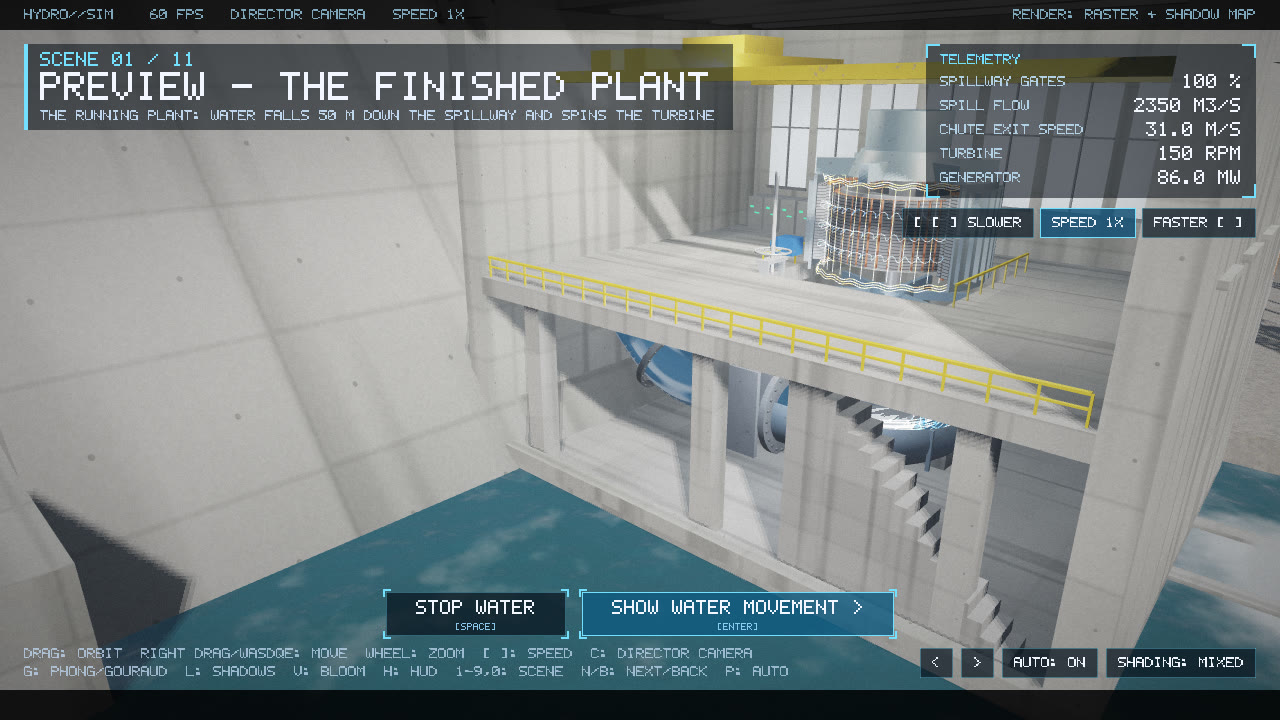
\includegraphics[width=0.70\textwidth]{01_preview_running_plant.jpg}
\caption{Scene 1: the running plant with the cut-away powerhouse.}
\label{fig:s1}
\end{figure}

\section{Scenes 2 and 3: Reservoir, Trash Rack and Intake Gate}

In scene 2 the camera flies over the dam crest and dives under the reservoir surface,
where the lighting changes to blue under-water light with caustics and drifting dust.
A dissolve leads to a cut-away of the trash rack. Branches, logs and plastic drift in
with the current and stop at the bars, while small leaves slip through
(Figure~\ref{fig:s23}a). The telemetry counts the trapped and passed pieces.

In scene 3 the dam block lifts away to reveal the intake gate. When it opens, the jet
under the gate shoots into the conduit at about 18\,m/s and the conduit fills. The
button to follow the water stays grey until the gate is fully open
(Figure~\ref{fig:s23}b).

\begin{figure}[H]
\centering
\begin{subfigure}[t]{0.49\textwidth}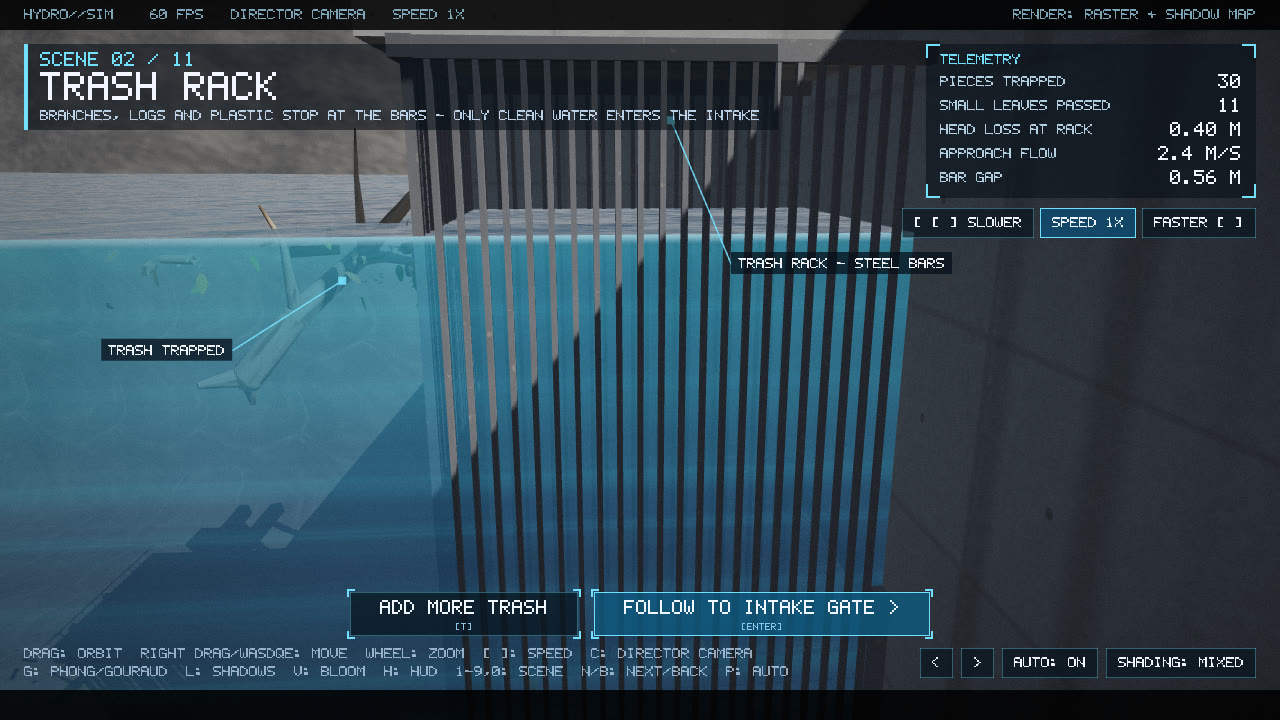
\includegraphics[width=\linewidth]{04_trash_rack_filtering.jpg}\caption{Trash stopped at the rack.}\end{subfigure}\hfill
\begin{subfigure}[t]{0.49\textwidth}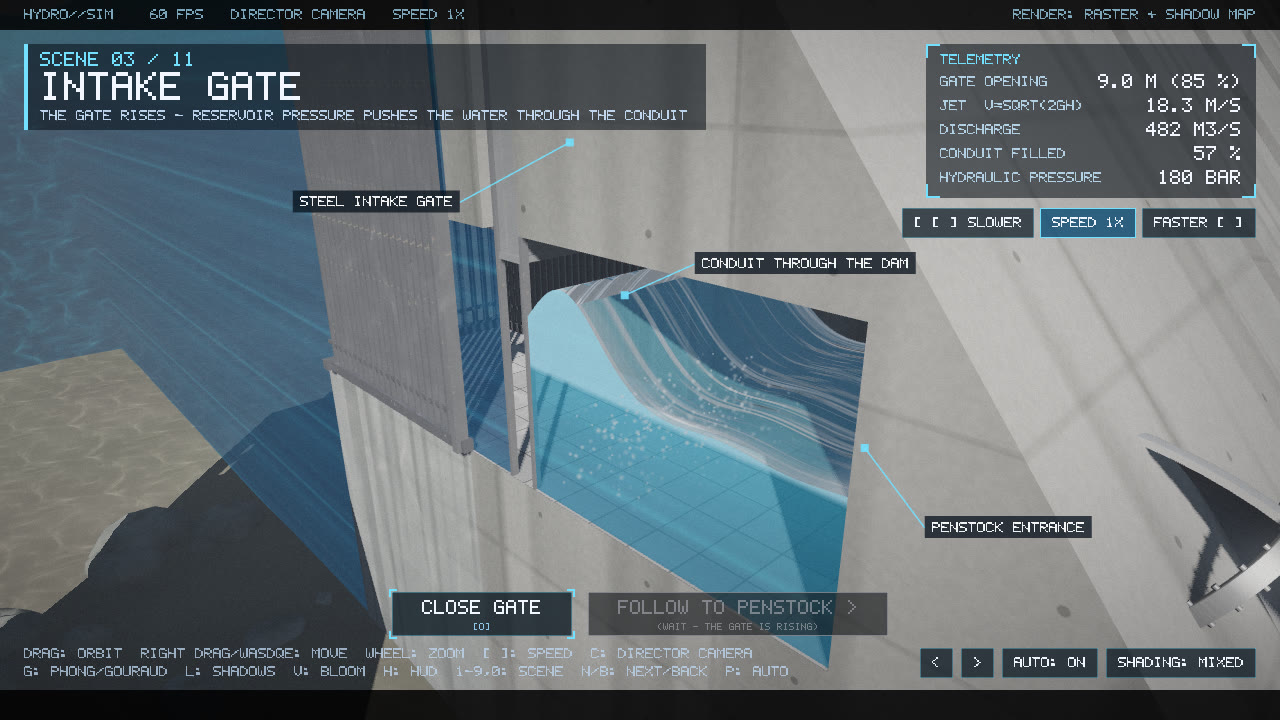
\includegraphics[width=\linewidth]{05_intake_gate_opening.jpg}\caption{The intake gate rising; water fills the conduit.}\end{subfigure}
\caption{Scenes 2 and 3.}
\label{fig:s23}
\end{figure}

\section{Scenes 4 and 5: Penstock and Ray-Traced Pipe}

The water rushes down the open penstock and accelerates as it drops
(Figure~\ref{fig:s45}a). Half way down the pipe switches to a glowing X-ray grid, and
at the bottom the water stops at the closed main inlet valve. A dissolve
then leads into the ray-traced scene (Figure~\ref{fig:s45}b), where the glass pipe
reflects in the floor, casts a blue shadow and shows glowing streams inside.

\begin{figure}[H]
\centering
\begin{subfigure}[t]{0.49\textwidth}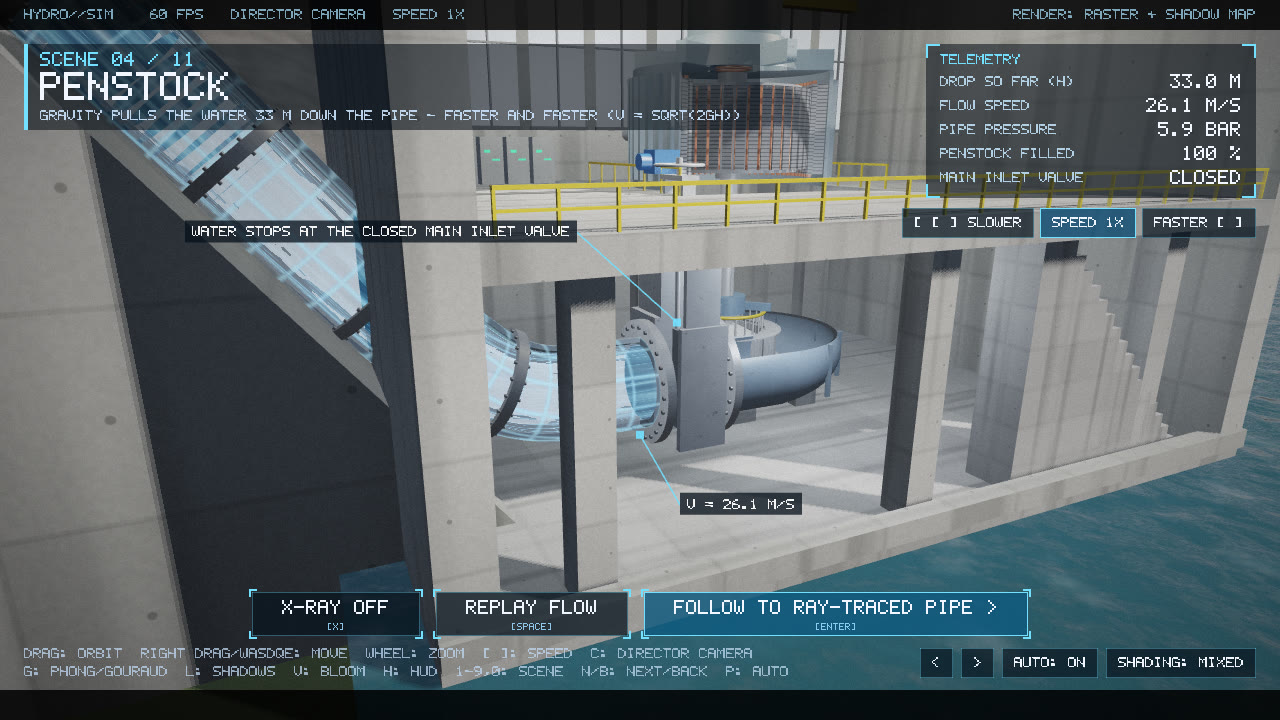
\includegraphics[width=\linewidth]{06_penstock_water_rushing.jpg}\caption{Water rushing down the penstock.}\end{subfigure}\hfill
\begin{subfigure}[t]{0.49\textwidth}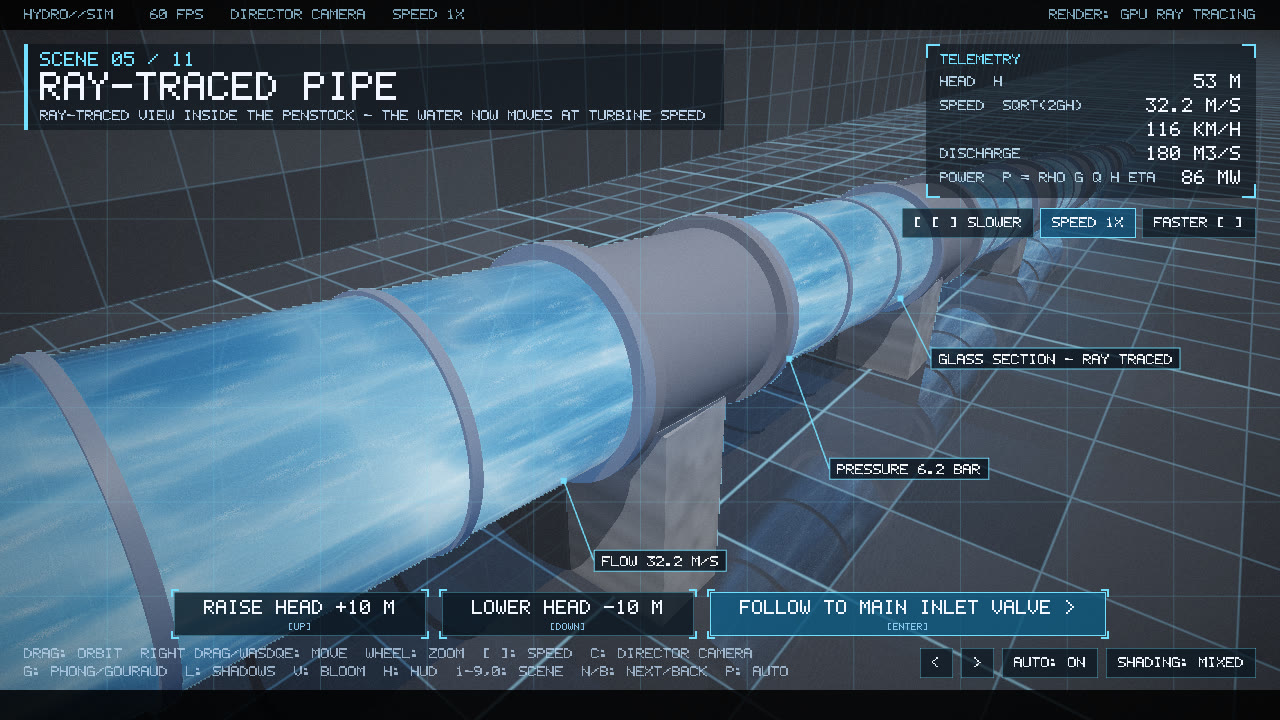
\includegraphics[width=\linewidth]{07_raytraced_pipe.jpg}\caption{The ray-traced penstock.}\end{subfigure}
\caption{Scenes 4 and 5.}
\label{fig:s45}
\end{figure}

\section{Scenes 6 and 7: Main Inlet Valve and Francis Turbine}

Opening the valve turns the hand-wheel and lifts the gate, and the water moves on into
the spiral casing (Figure~\ref{fig:s67}a). In scene 7 the camera looks down into the
open casing: blue streamlines swirl round it, pass between the stay and guide vanes and
enter the runner (Figure~\ref{fig:s67}b). Opening the guide vanes lets the water in, and
the runner speeds up with inertia towards 150\,rpm while the telemetry shows flow,
torque and mechanical power. The section view (Figure~\ref{fig:s7sec}) shows the water
turning down through the runner into the draft tube.

\begin{figure}[H]
\centering
\begin{subfigure}[t]{0.49\textwidth}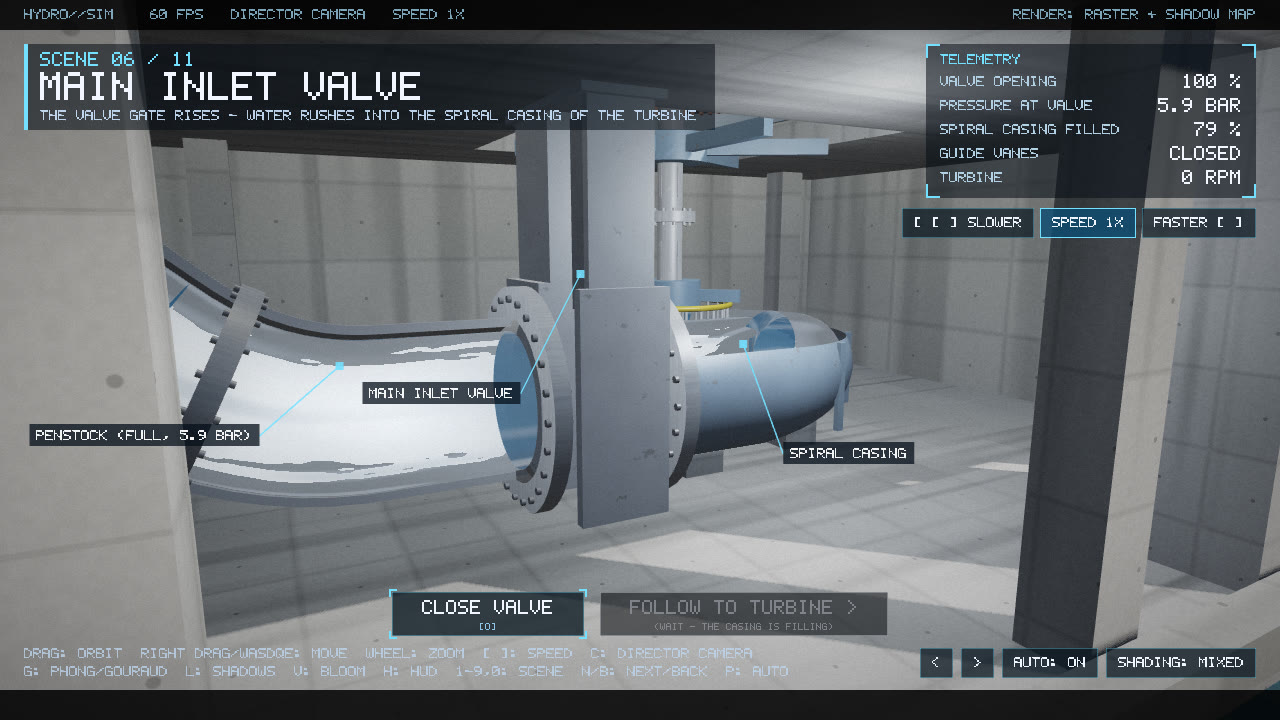
\includegraphics[width=\linewidth]{08_main_inlet_valve_open.jpg}\caption{The main inlet valve; the casing is filling.}\end{subfigure}\hfill
\begin{subfigure}[t]{0.49\textwidth}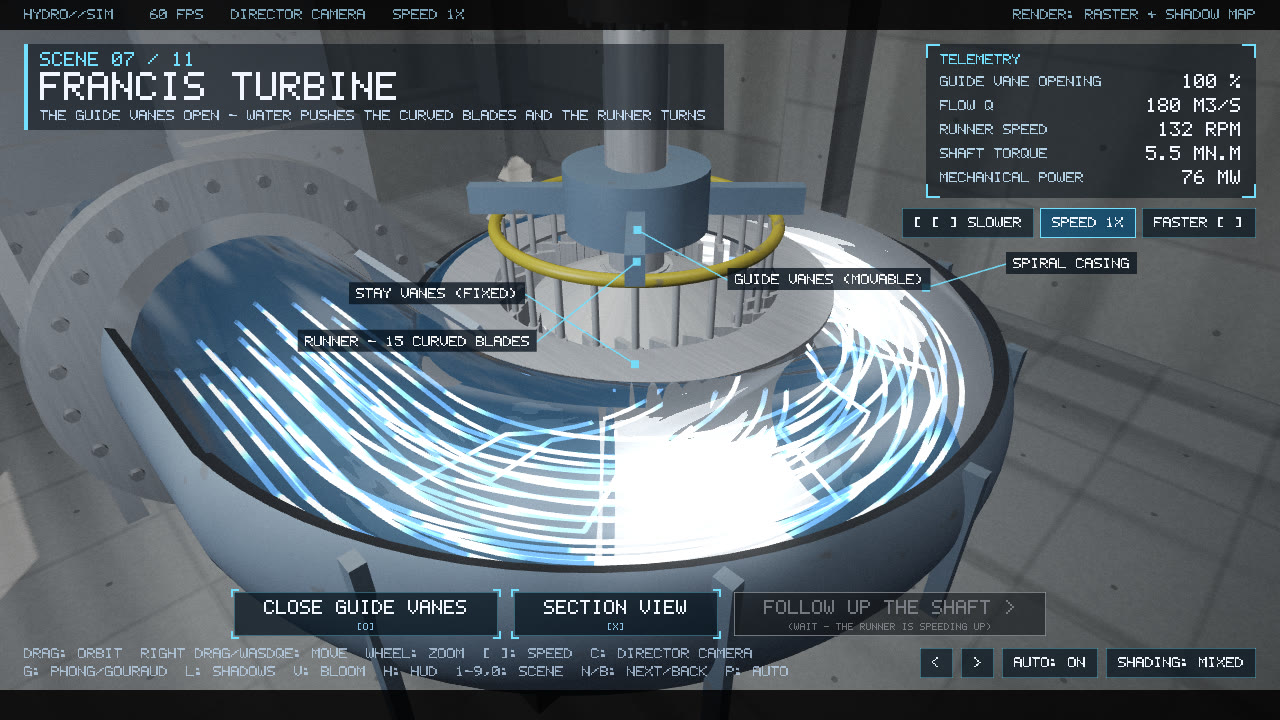
\includegraphics[width=\linewidth]{09_turbine_top_view.jpg}\caption{Top view of the spiral casing and vanes.}\end{subfigure}
\caption{Scenes 6 and 7.}
\label{fig:s67}
\end{figure}

\begin{figure}[H]
\centering
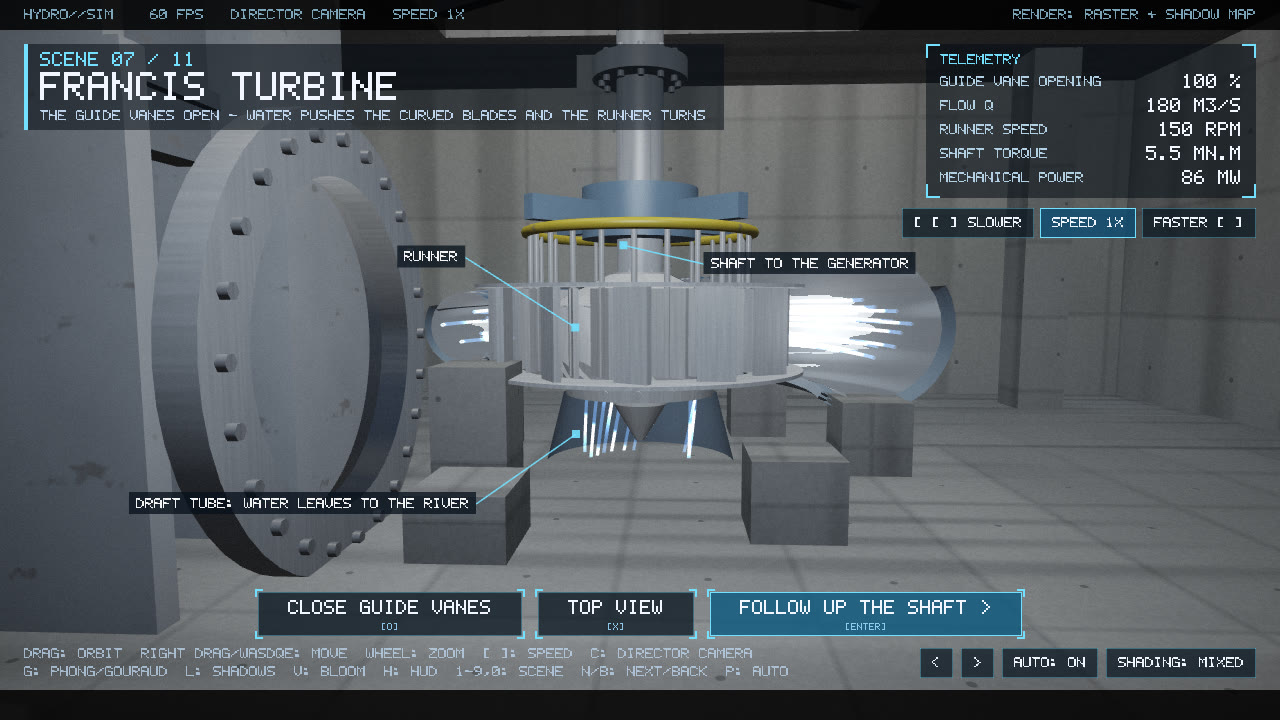
\includegraphics[width=0.62\textwidth]{10_turbine_section_view.jpg}
\caption{Section view of the Francis turbine with the streamlines leaving through the draft tube.}
\label{fig:s7sec}
\end{figure}

\section{Scenes 8 and 9: Shaft and Generator}

Scene 8 is an automatic hologram-style rise along the turning shaft, past the guide
bearing and the coupling flange, to the generator. In scene 9 (Figure~\ref{fig:s89})
the viewer excites the rotor. The field current rises, magnetic field lines appear,
orange current pulses run through the stator coils, and the oscilloscope shows the
three phases growing to 11\,kV at 50\,Hz.

\begin{figure}[H]
\centering
\begin{subfigure}[t]{0.49\textwidth}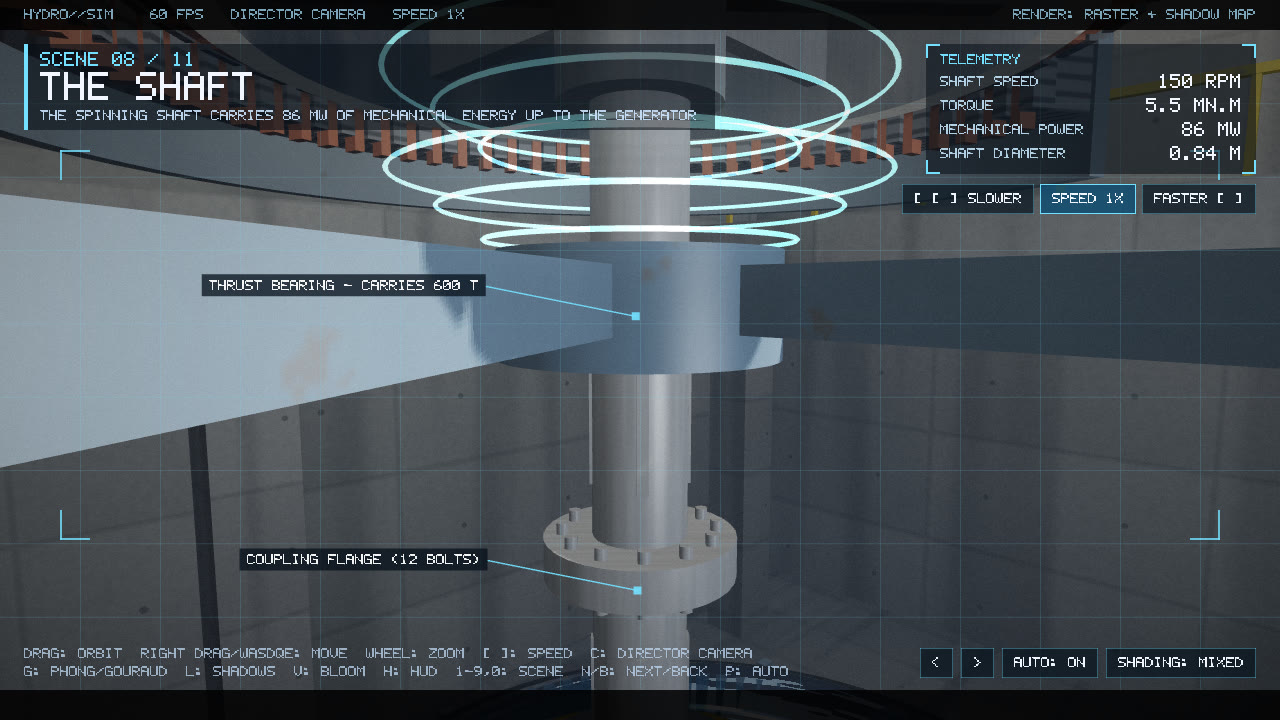
\includegraphics[width=\linewidth]{11_shaft_hologram_rise.jpg}\caption{Scene 8: the shaft and coupling flange.}\end{subfigure}\hfill
\begin{subfigure}[t]{0.49\textwidth}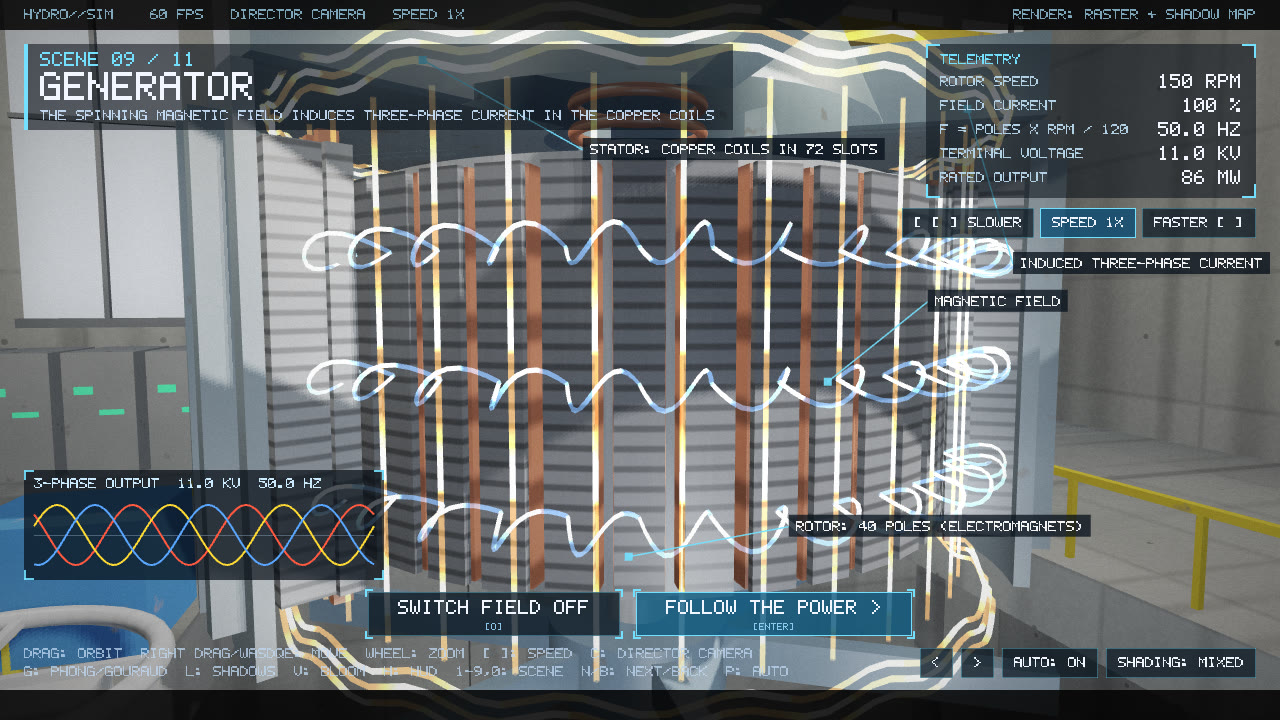
\includegraphics[width=\linewidth]{12_generator_excited.jpg}\caption{Scene 9: the excited generator and oscilloscope.}\end{subfigure}
\caption{Scenes 8 and 9.}
\label{fig:s89}
\end{figure}

\section{Scenes 10 and 11: Transformer and Grid}

The camera flies out over the powerhouse roof to the transformer yard. The bus ducts
glow with current, and the X-ray view shows the windings inside the tank
(Figure~\ref{fig:s1011}a). In the switchyard the disconnector, breaker, current
transformers and surge arresters are labelled. Closing the breaker sends the energy
along the power line, and the camera flies with it to the horizon
(Figure~\ref{fig:s1011}b). At the end, a summary of the whole energy chain appears
(Figure~\ref{fig:summary}), and \textsc{Replay journey} returns to the preview.

\begin{figure}[H]
\centering
\begin{subfigure}[t]{0.49\textwidth}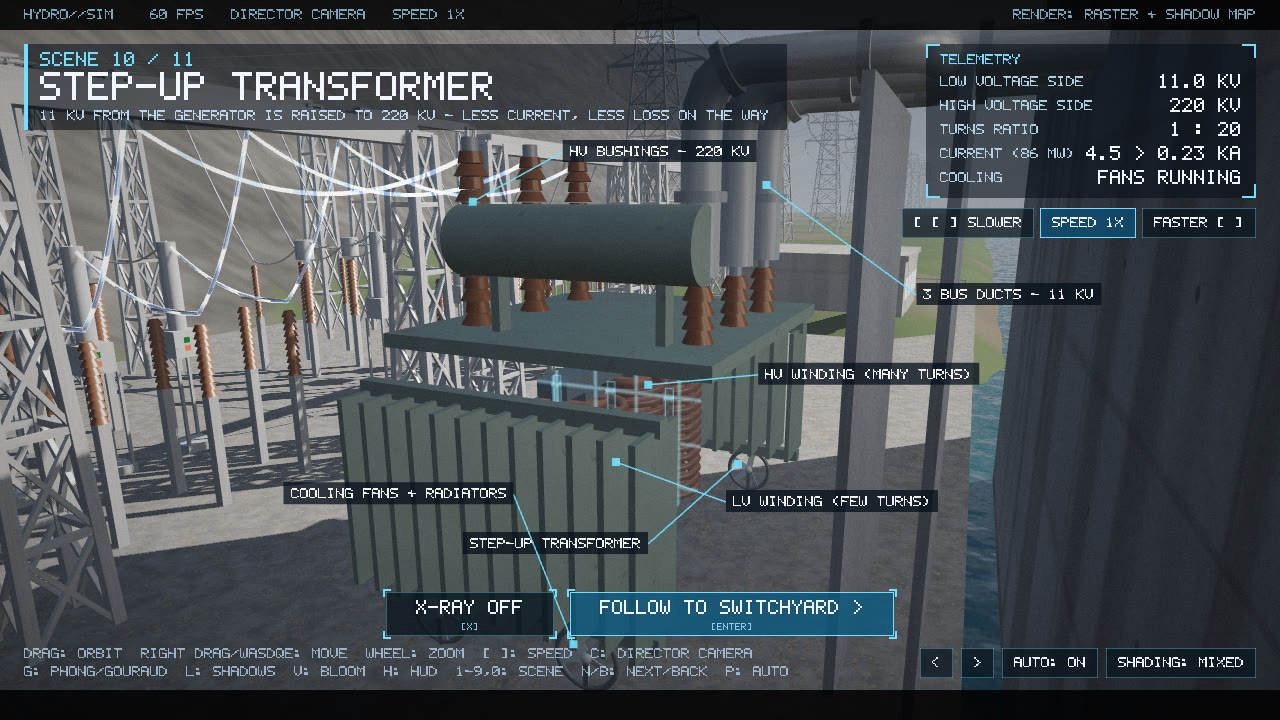
\includegraphics[width=\linewidth]{13_transformer_xray.jpg}\caption{Scene 10: transformer in X-ray view.}\end{subfigure}\hfill
\begin{subfigure}[t]{0.49\textwidth}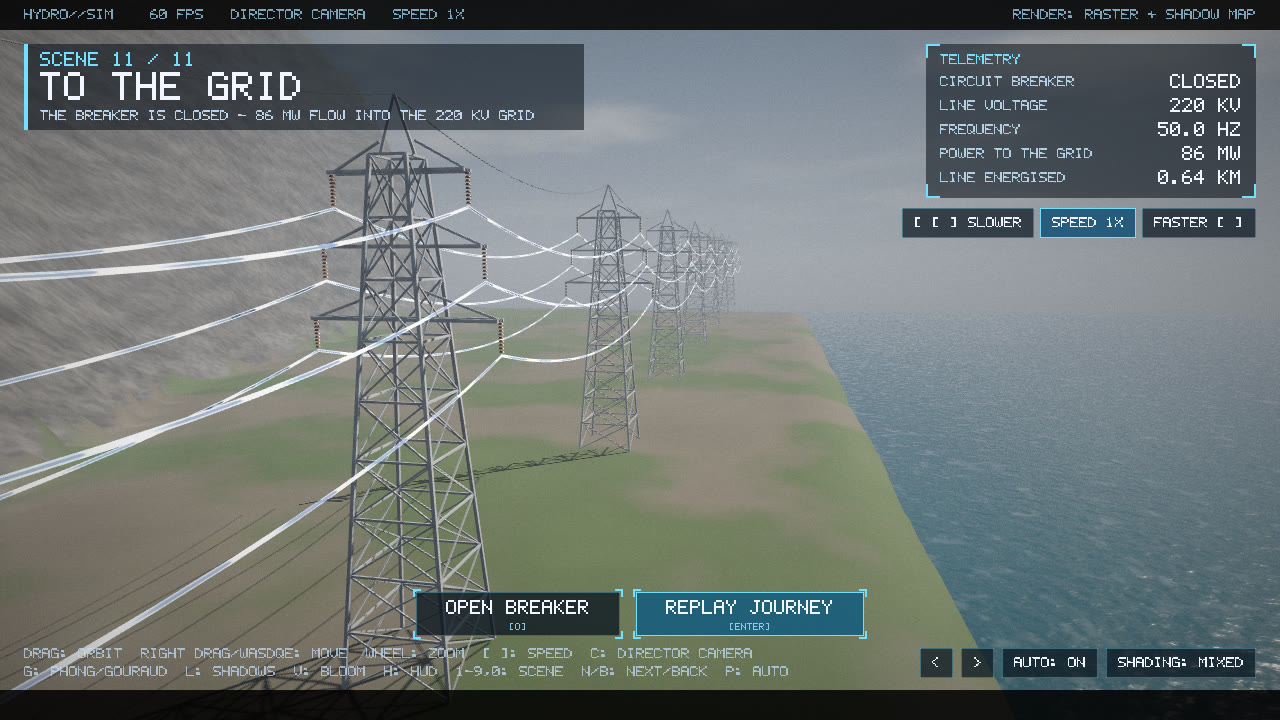
\includegraphics[width=\linewidth]{15_power_along_the_line.jpg}\caption{Scene 11: energy travelling along the line.}\end{subfigure}
\caption{Scenes 10 and 11.}
\label{fig:s1011}
\end{figure}

\begin{figure}[H]
\centering
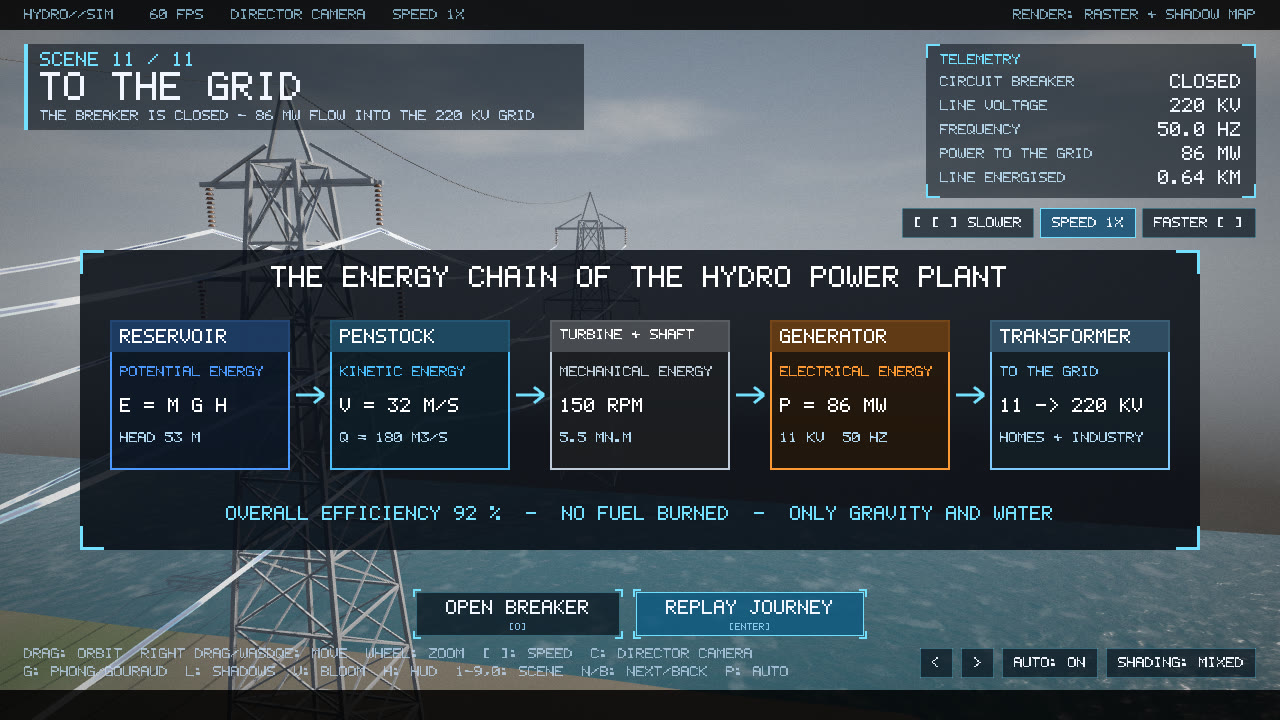
\includegraphics[width=0.70\textwidth]{16_energy_chain_summary.jpg}
\caption{The energy-chain summary at the end of the journey.}
\label{fig:summary}
\end{figure}

% =====================================================================
%  CHAPTER 7  RESULTS
% =====================================================================
\chapter{Results, Testing and Discussion}
\label{ch:results}

\section{Main Results}

The final program meets all the goals set in Chapter~1. It presents the whole plant,
from reservoir to grid, as one continuous, interactive world, demonstrates
all six compulsory topics (Table~\ref{tab:req}), and implements every object and
feature of the proposal in the context of a hydroelectric plant
(Tables~\ref{tab:objects} and~\ref{tab:features}). The plant is built from 18 object
files and runs in 11 connected scenes, and apart from GLFW and GLAD every piece of
maths, geometry and texture is the project's own code.

\section{Testing Method}

A graphics program has to be checked by looking at it, so the program includes tools
that make looking repeatable:

\begin{itemize}
  \item \textbf{Shot mode} (\code{--shot <scene> <seconds> <file>}) starts a scene,
        runs the story for a fixed simulated time at a fixed time step, and saves a
        picture. Button presses can be scripted with \code{--press}. Every figure in this
        report was made this way, which also means any figure can be reproduced exactly.
  \item \textbf{Automatic test} (\code{--autotest}) runs the real frame loop on AUTO,
        including the dissolves. The full chain reaches the energy summary at about 180
        seconds.
  \item \textbf{Benchmark} (\code{--bench}) measures the real frame time of every scene.
  \item Switches \code{--shading}, \code{--noshadows} and \code{--nopost} produce the
        matched comparison images of Chapter~\ref{ch:theory}.
\end{itemize}

\section{Performance}
\label{sec:perf}

The plant contains far more detail than any one view shows, so the world culls what
cannot be seen. The detailed machines (valve, turbine, generator) are drawn only when
the camera is within 160\,m of the powerhouse, and the transformer, switchyard and
power line are skipped while the camera is inside the hall. Meshes are built once and
reused: one guide-vane mesh is drawn 24 times and one spillway-gate mesh three times.
Bloom works at a quarter of the screen size, and particles live in a fixed-capacity
array with constant-time removal.

Table~\ref{tab:fps} gives the measured frame rates at 1600$\times$900 on a laptop with
an NVIDIA GeForce GTX~1650. Every scene stays above the 30 frames per second usually
needed for smooth motion. The ray-traced scene is the most expensive, because each
pixel traces several rays and marches 36 steps through the water.

\begin{table}[!htbp]
\centering
\caption{Measured performance at 1600$\times$900 (GTX 1650).}
\label{tab:fps}
\begin{tabular}{@{}rlrr@{}}
\toprule
\textbf{\#} & \textbf{Scene} & \textbf{ms / frame} & \textbf{fps} \\
\midrule
1 & Preview & 26.6 & 37.5 \\
2 & Reservoir and trash rack & 18.7 & 53.6 \\
3 & Intake gate & 20.2 & 49.4 \\
4 & Penstock & 20.6 & 48.6 \\
5 & Ray-traced pipe & 29.3 & 34.1 \\
6 & Main inlet valve & 23.7 & 42.2 \\
7 & Francis turbine & 22.8 & 43.8 \\
8 & Shaft & 22.7 & 44.0 \\
9 & Generator & 27.0 & 37.0 \\
10 & Transformer & 18.8 & 53.1 \\
11 & Switchyard and grid & 16.6 & 60.4 \\
\bottomrule
\end{tabular}
\end{table}

\section{Limitations}

\begin{itemize}
  \item The interiors are cut-away teaching diagrams, not fully closed engineering
        models.
  \item The physics is simplified for teaching. Water fronts follow free-fall and
        Torricelli formulas rather than a fluid simulation, and the water is shown slower
        than real speed so the eye can follow it.
  \item The plant has a single turbine--generator unit.
  \item Ray tracing is used for the penstock scene only; the rest of the world is
        rasterised. Shadow rays in the ray tracer produce hard shadows.
  \item Only the sun casts shadows; the point lights in the powerhouse do not.
  \item There is no sound.
\end{itemize}

% =====================================================================
%  CHAPTER 8  CONCLUSION
% =====================================================================
\chapter{Conclusion and Future Work}
\label{ch:conclusion}

\section{Conclusion}

What started as a small sluice-gate scene became a complete hydroelectric power plant
that can be explored from the reservoir to the power line. The project uses plain
OpenGL and C++, with every shape, texture and matrix written from scratch. It
demonstrates lighting with ambient, diffuse and specular terms, every kind of
transformation, Gouraud and Phong shading side by side, continuous physics-based
animation, rich interaction, and a real ray tracer. On top of these it adds shadow
mapping, water rendering, particles, glowing flow lines and a post-processing pass that
give the scenes a cinematic look.

The part I am most satisfied with is that the program explains something real. The
numbers on screen come from real formulas and agree with each other, the machines only
move when their cause allows it, and the viewer learns the order of operation of a
power plant by operating it.

\section{Future Work}

\begin{itemize}
  \item Several turbine units with a control room that shares load between them.
  \item A simple fluid simulation for the spillway and the reservoir surface.
  \item Ray-traced reflections and soft shadows for the whole world, not only one scene.
  \item Shadows from the powerhouse lamps using cube shadow maps.
  \item Sound: rushing water, the hum of the generator, the click of the breaker.
  \item A day--night cycle with lights coming on along the transmission line.
\end{itemize}

% =====================================================================
%  REFERENCES
% =====================================================================
\begin{thebibliography}{99}
\addcontentsline{toc}{chapter}{References}

\bibitem{foley} J.~D. Foley, A.~van Dam, S.~K. Feiner, and J.~F. Hughes,
\emph{Computer Graphics: Principles and Practice}, 2nd~ed. Addison-Wesley, 1996.

\bibitem{rtr} T.~Akenine-M\"oller, E.~Haines, N.~Hoffman, A.~Pesce, M.~Iwanicki, and
S.~Hillaire, \emph{Real-Time Rendering}, 4th~ed. CRC Press, 2018.

\bibitem{phong} B.~T. Phong, ``Illumination for computer generated pictures,''
\emph{Communications of the ACM}, vol.~18, no.~6, pp.~311--317, 1975.

\bibitem{blinn} J.~F. Blinn, ``Models of light reflection for computer synthesized
pictures,'' \emph{Computer Graphics (Proc. SIGGRAPH '77)}, vol.~11, no.~2,
pp.~192--198, 1977.

\bibitem{gouraud} H.~Gouraud, ``Continuous shading of curved surfaces,'' \emph{IEEE
Transactions on Computers}, vol.~C-20, no.~6, pp.~623--629, 1971.

\bibitem{whitted} T.~Whitted, ``An improved illumination model for shaded display,''
\emph{Communications of the ACM}, vol.~23, no.~6, pp.~343--349, 1980.

\bibitem{williams} L.~Williams, ``Casting curved shadows on curved surfaces,''
\emph{Computer Graphics (Proc. SIGGRAPH '78)}, vol.~12, no.~3, pp.~270--274, 1978.

\bibitem{reeves87} W.~T. Reeves, D.~H. Salesin, and R.~L. Cook, ``Rendering antialiased
shadows with depth maps,'' \emph{Computer Graphics (Proc. SIGGRAPH '87)}, vol.~21,
no.~4, pp.~283--291, 1987.

\bibitem{schlick} C.~Schlick, ``An inexpensive BRDF model for physically-based
rendering,'' \emph{Computer Graphics Forum}, vol.~13, no.~3, pp.~233--246, 1994.

\bibitem{catmull} E.~Catmull and R.~Rom, ``A class of local interpolating splines,'' in
\emph{Computer Aided Geometric Design}, R.~E. Barnhill and R.~F. Riesenfeld, Eds.
Academic Press, 1974, pp.~317--326.

\bibitem{reeves83} W.~T. Reeves, ``Particle systems---a technique for modeling a class
of fuzzy objects,'' \emph{ACM Transactions on Graphics}, vol.~2, no.~2, pp.~91--108,
1983.

\bibitem{iq} I.~Quilez, ``Ray--surface intersectors.''
\url{https://iquilezles.org/articles/intersectors/}

\bibitem{hoskins} D.~Hoskins, ``Hash without sine,'' Shadertoy.
\url{https://www.shadertoy.com/view/4djSRW}

\bibitem{caustic} ``Tileable water caustic,'' Shadertoy.
\url{https://www.shadertoy.com/view/MdlXz8}

\bibitem{aces} K.~Narkowicz, ``ACES filmic tone mapping curve,'' 2016.
\url{https://knarkowicz.wordpress.com/2016/01/06/aces-filmic-tone-mapping-curve/}

\bibitem{learnopengl} J.~de~Vries, \emph{Learn OpenGL}. \url{https://learnopengl.com}

\bibitem{glspec} M.~Segal and K.~Akeley, \emph{The OpenGL Graphics System: A
Specification (Version 3.3, Core Profile)}. Khronos Group, 2010.

\bibitem{glslspec} J.~Kessenich, \emph{The OpenGL Shading Language, Version 3.30}.
Khronos Group, 2010.

\bibitem{white} F.~M. White, \emph{Fluid Mechanics}, 7th~ed. McGraw-Hill, 2011.

\bibitem{chapman} S.~J. Chapman, \emph{Electric Machinery Fundamentals}, 5th~ed.
McGraw-Hill, 2012.

\end{thebibliography}

% =====================================================================
%  APPENDICES
% =====================================================================
\appendix

\chapter{The Approved Proposal}
\label{app:proposal}

Figure~\ref{fig:proposal} shows the original proposal. The teacher's note
``Hydroelectric Power Plant'' at the top asked for the sluice-gate idea to be grown into
a hydroelectric power plant simulation, which is the project described in this report.

\begin{figure}[!htbp]
\centering
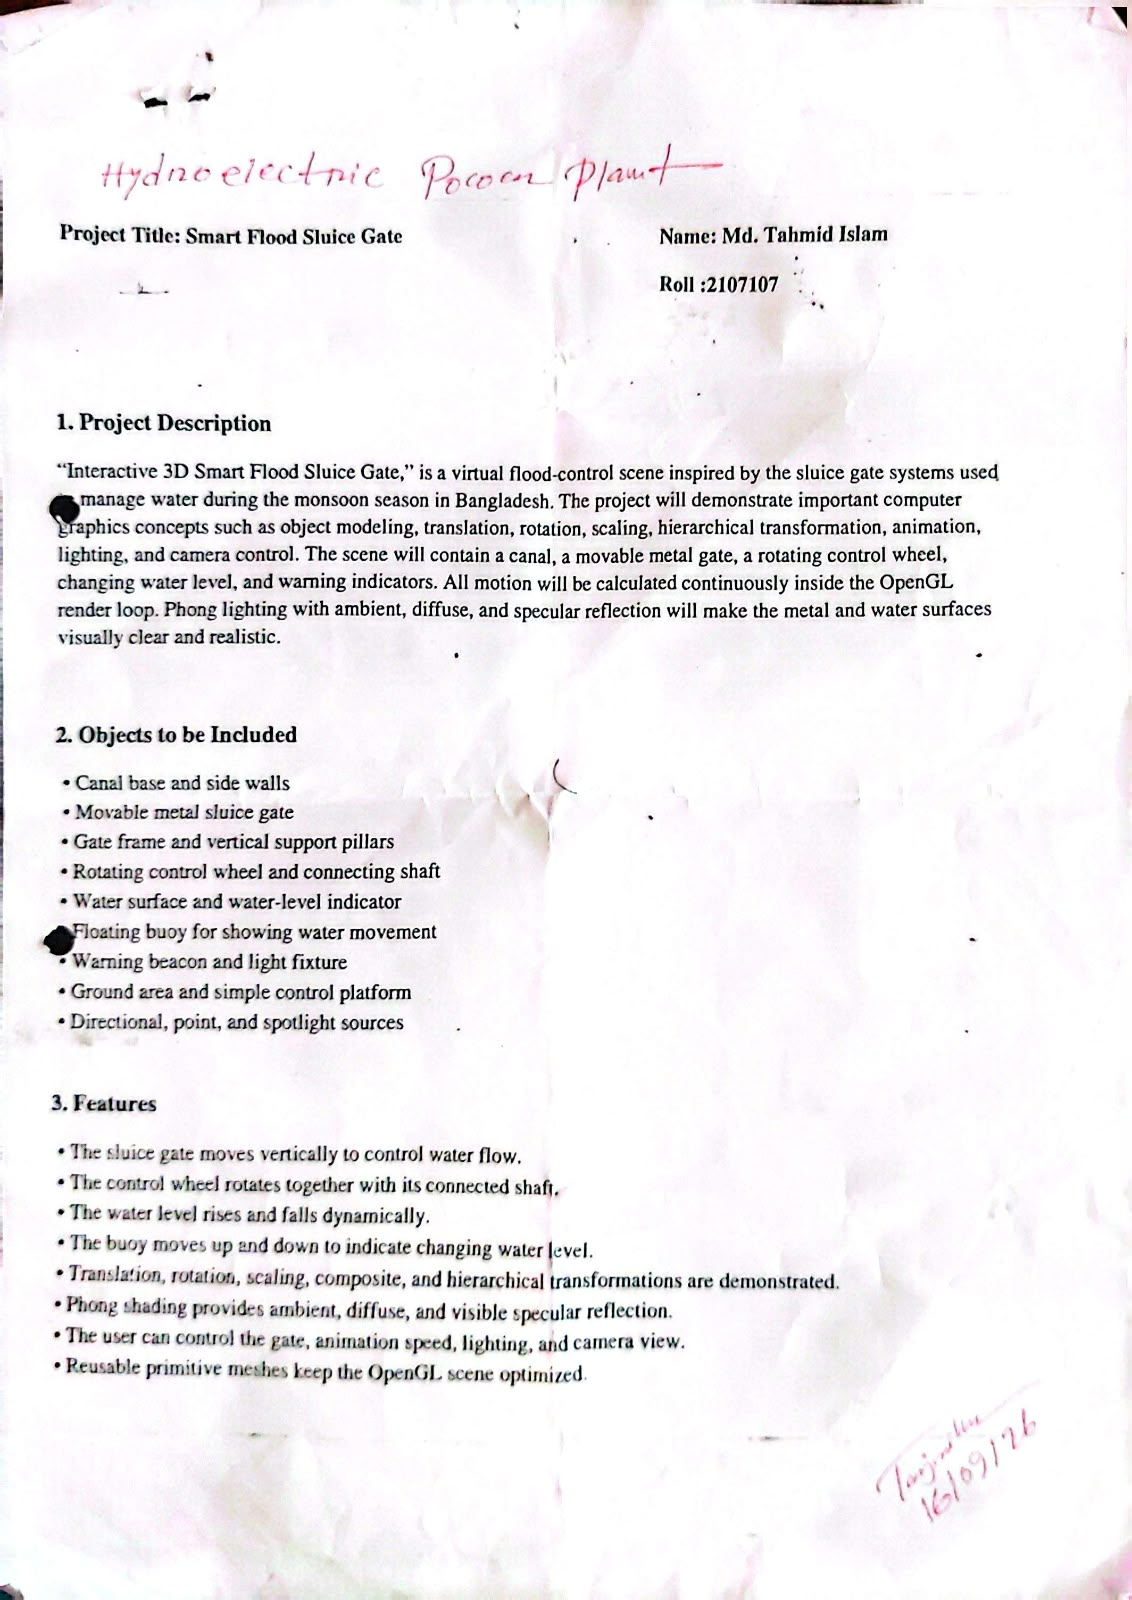
\includegraphics[width=0.74\textwidth]{ProposedNew.jpeg}
\caption{The original proposal, \emph{Smart Flood Sluice Gate}, with the teacher's note.}
\label{fig:proposal}
\end{figure}

\chapter{Building and Running the Program}

\section*{Source code}
The complete source code of the project is available on GitHub:\\
\url{https://github.com/tahmidalbi/Hydro-electric-Powerplant-Simulation-with-OpenGL}

\section*{Requirements}
Windows with MSYS2 MinGW-w64 installed at \texttt{C:\textbackslash msys64\textbackslash mingw64} (including the GLFW
package), and a graphics card with OpenGL~3.3.

\section*{Building and running}
\begin{itemize}
  \item Double-click \code{run.bat}. It builds the program the first time and then
        starts it.
  \item Or open a terminal inside the project folder. \code{build.bat} compiles the
        program, and \code{run.bat} starts it. The program itself is
        \texttt{build\textbackslash hydro.exe}.
\end{itemize}

\section*{Command-line options}
\begin{tabularx}{\textwidth}{@{}L{5.6cm}Y@{}}
\toprule
\textbf{Option} & \textbf{Effect} \\
\midrule
\code{--size 1920 1080} & Window size \\
\code{--nopost} & Start without bloom, vignette and grain \\
\code{--noshadows} & Start with shadows off \\
\code{--shading phong|gouraud} & Start in the given shading mode \\
\code{--bench} & Print the frame time of every scene \\
\code{--shot 7 19 pic.bmp} & Start scene 7, run 19\,s on AUTO, save a picture \\
\code{--autotest 60 pic.bmp} & Run the real frame loop on AUTO for 60\,s, then save a picture \\
\bottomrule
\end{tabularx}

\section*{Project folder}
\noindent\begin{minipage}{\linewidth}
\begin{lstlisting}[language={}]
HYDRO/
  build.bat, run.bat, CMakeLists.txt
  shaders/        21 GLSL files: lighting, water, sky, particles, ray tracer,
                  flow lines, post-processing, HUD
  src/
    main.cpp      command line
    App.cpp/.h    window, input, transitions, speed control, HUD
    core/         MathLib, Mesh + MeshBuilder, Shader, Camera, Screenshot
    render/       Renderer, ParticleSystem, FrameCapture, PostFX
    objects/      one file per object + World + PlantData
    scenes/       Scene1_Preview ... Scene11_Grid
    ui/           pixel Font, Ui
  docs/           technical notes
  captures/       pictures rendered by the program
  report/         this report
\end{lstlisting}
\end{minipage}

\end{document}
